\chapter{Sistemas continuos}

En este cap'itulo aprenderemos c'omo cuantizar un sistema con un continuo de
grados de libertad, tal como el campo electromagn'etico. Para tal efecto
comenzaremos recordando algunos aspectos de las formulaciones Lagrangeana y
Hamiltoniana de la Mec'anica. En particular, estudiaremos un sistema f'isico
compuesto de un n'umero finito de part'iculas que interact'uan por medio de un
potencial arm'onico y que est'an restringidas a moverse en una linea recta.
Luego,
investigaremos las expresiones obtenidas en este estudio en el l'imite de un
n'umero infinito de part'iculas, para llegar as'i al concepto de campo.

\section{Cadena lineal cl'asica}

\subsection{Modelo discreto}

Consideremos un sistema f'isico constituido por part'iculas de igual masa que 
interact'uan s'olo con sus primeros vecinos por medio de una fuerza arm'onica.
Este sistema se denomina ``Cadena lineal cl'asica". Este sistema puede ser
considerado como un modelo (muy) simplificado de un s'olido (unidimensional),
donde las masas representan 'atomos de la red que forman el s'olido y los
resortes modelan las interacciones entre los 'atomos individuales.

En condiciones de equilibrio las part'iculas se encuentran separadas por una
distancia $\Delta x^{l}$, donde $l=1,\dots, N$ es el 'indice que individualiza a
cada una de las part'iculas. La fuerza arm'onica est'a caracterizada por una
constante $k$. Denotaremos con $q^{l}$ al desplazamiento de la part'icula
$l$-esima con respecto a su posici'on de equilibrio.
\begin{figure}
	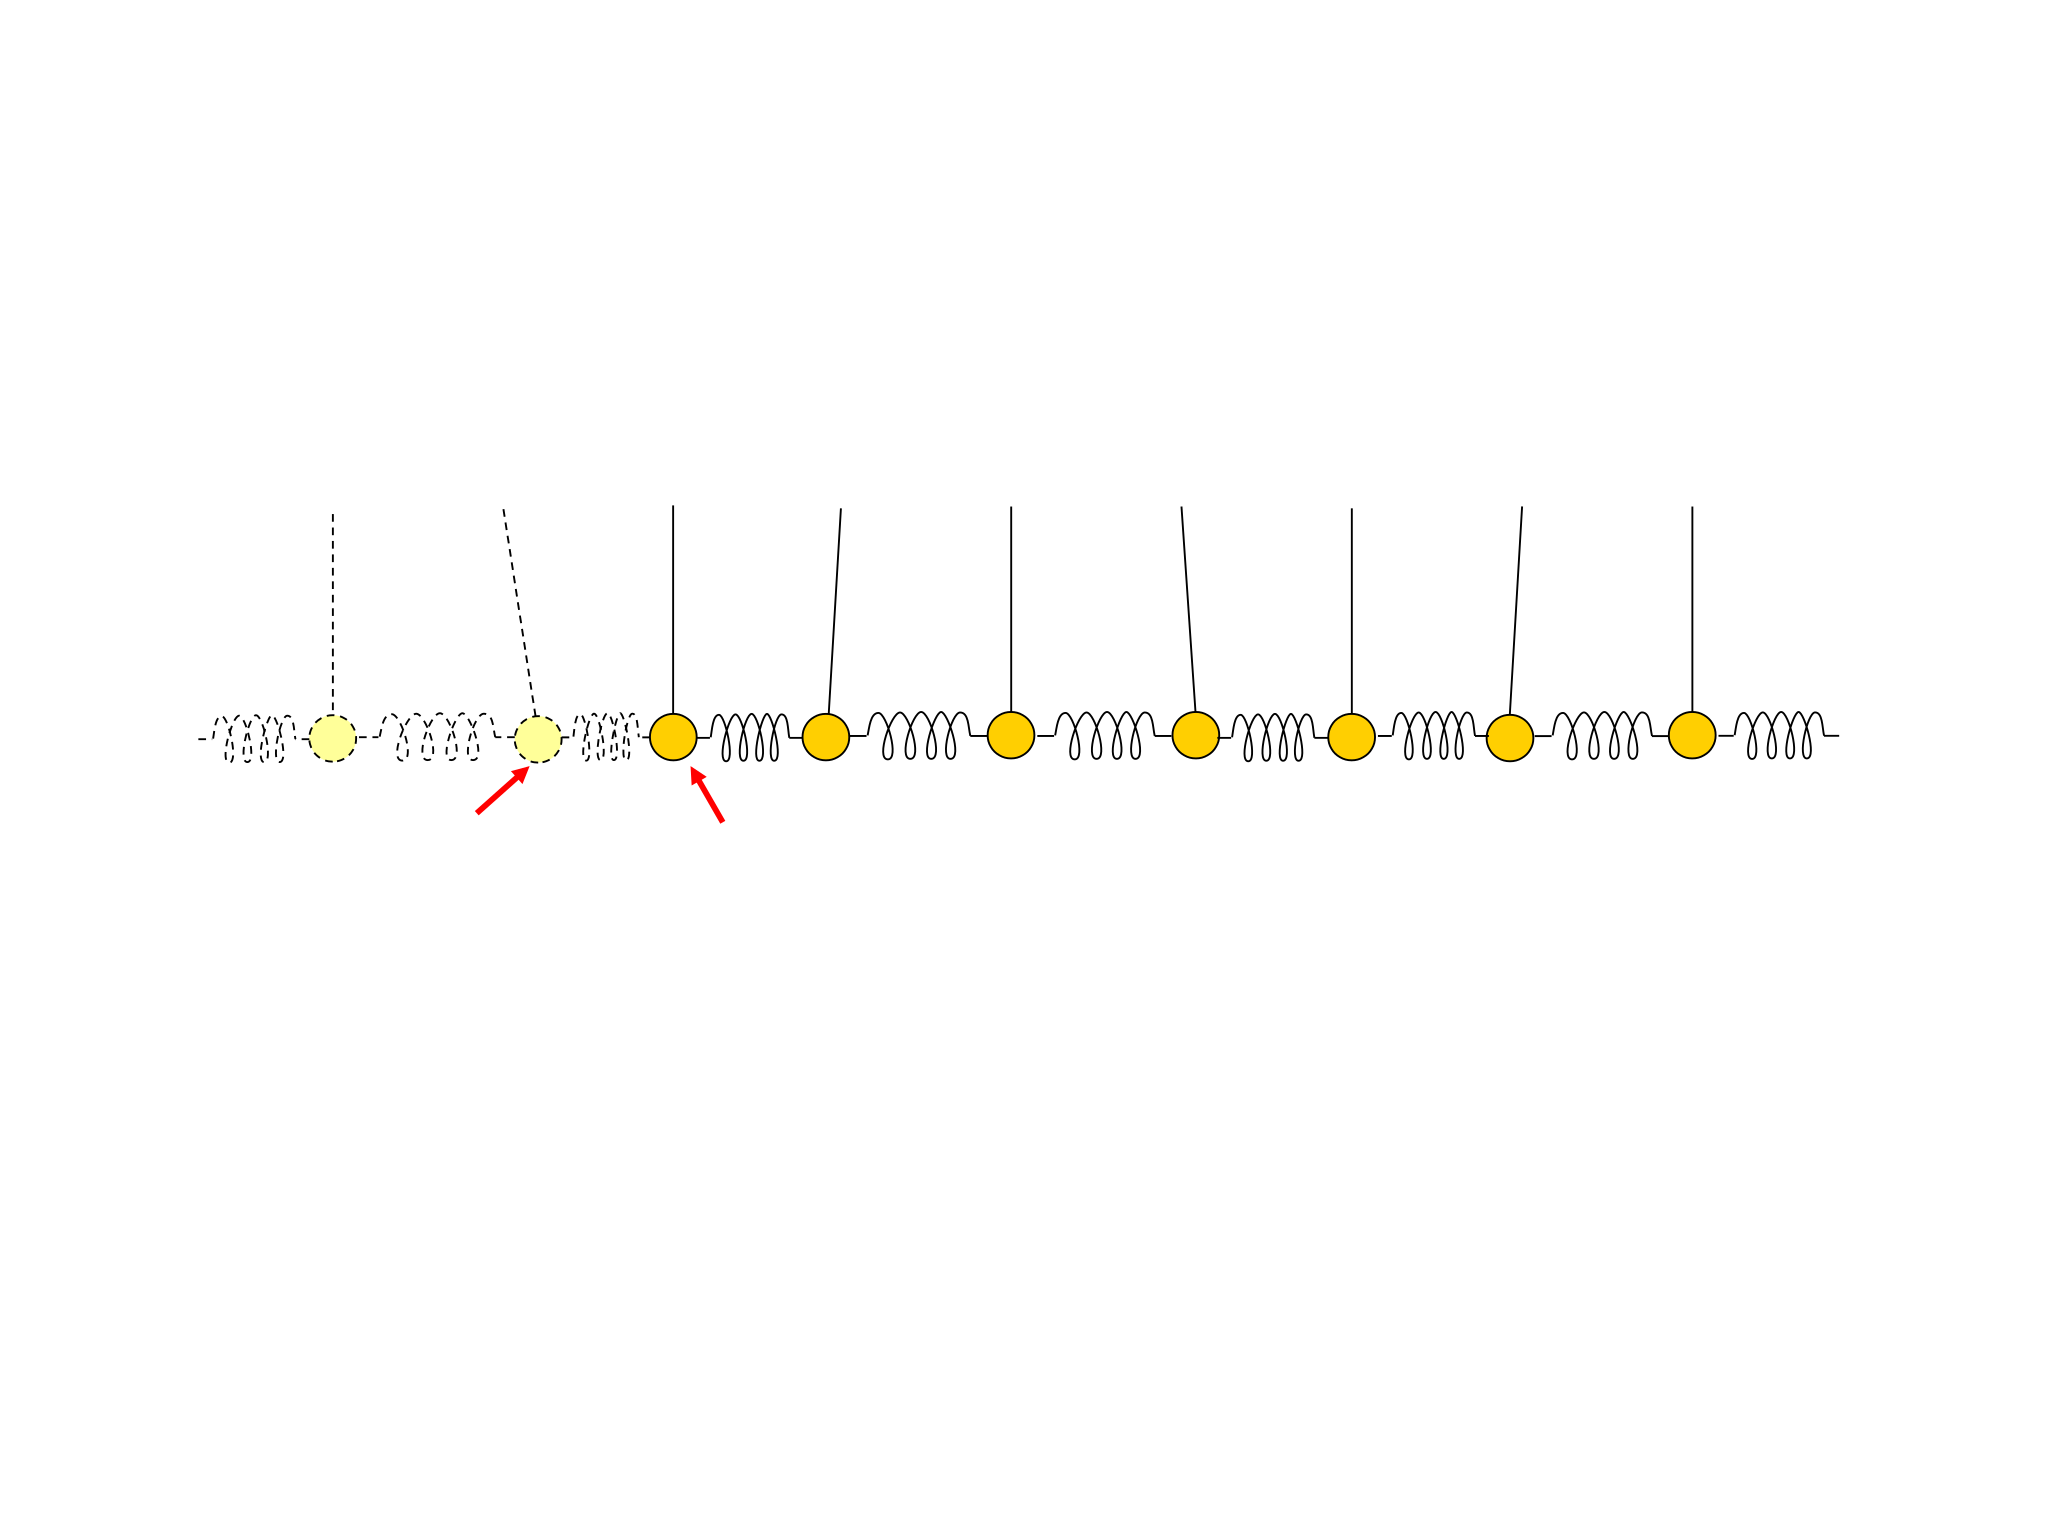
\includegraphics[height=4cm]{figs/fig-cadena.pdf}
	\caption{Cadena lineal.}
	\label{fig:cadena}
\end{figure}
La energ'ia cin'etica $T$ de este sistema est'a dada por:
\begin{equation}
T=\frac{1}{2}\sum_{l=1}^{N}m(\dot{q}^{l})^{2}(t).
\end{equation}
La energ'ia potencial $V$, que corresponde a la suma de las energ'ias
potenciales asociadas a cada una de las fuerzas arm'onicas, es
\begin{equation}
V=\frac{1}{2}\sum_{l=1}^{N}k\left\{ q^{l+1}(t) -q^{l}\left(
t\right) \right\} ^{2}.
\end{equation}
Por lo tanto, el Lagrangeano del sistema es
\begin{eqnarray}
L & = &T-V\\
& = &\frac{1}{2}\sum_{l=1}^{N}m(\dot{q}^{l})^{2}(t) -\frac{1}{2}
\sum_{l=1}^{N}k\left\{ q^{l+1}(t) -q^{l}(t)
\right\} ^{2}\\
& = &\frac{1}{2}\sum_{l=1}^{N}\left[ m(\dot{q}^{l})^{2}(t)
-k\left\{ q^{l+1}(t) -q^{l}(t) \right\}
^{2}\right].
\label{CLC}
\end{eqnarray}

\subsection{Ecuaciones de movimiento y soluci'on}
Las ecuaci'ones de movimiento de un sistema con $N$ grados de libertad pueden
ser obtenidas a partir de un lagrangeano $L=L\left(
q^{l},\dot{q}^{l}\right) $ mediante las ecuaciones de
Euler-Lagrange, esto es
\begin{equation}
\frac{\delta L}{\delta q^l}=\frac{\partial L}{\partial q^{l}}-\frac{d}{dt}\left(
\frac{\partial L}{\partial\dot{q}^{l}}\right) =0\label{EcMov1},
\end{equation}
donde hay una ecuaci'on para cada coordenada generalizada (o grado de libertad)
$q^{l}$, con $l=1,2,\dots,N$.

Considerando que para el Lagrangeano de la cadena lineal cl'asica tenemos
\begin{equation}
\frac{\partial L}{\partial\dot{q}^{l}}=m\dot{q}^l, \qquad \frac{\partial
L}{\partial q^{l}}=k(q^{l+1}-q^l)-k(q^l-q^{l-1})=k(q^{l+1}-2q^l+q^{l-1}),
\end{equation}
obtenemos que las ecuaciones de movimiento son:
\begin{equation}
\ddot{q}^l=g(q^{l+1}-2q^l+q^{l-1}).
\label{ecmovcl}
\end{equation}
Notese que hemos definido $g:=k/m$.

Para encontrar la soluci'on de las ecuaciones (\ref{ecmovcl}) es conveniente
suponer que los modos de vibraci'on de la cadena pueden ser descritos por una
onda plana. Esto est'a sugerido por la forma de la ecuaci'on (\ref{ecmovcl}),
puesto que si omitimos el primer y tercer t'ermino del miembro derecho obtenemos
la ecuaci'on del oscilador arm'onico. Adem'as, siempre podemos considerar una
expansi'on en serie de Fourier de las coordenadas generalizadas. Luego,
asumiremos una soluci'on de la forma
\begin{equation}
q^l(t)=B_k(t) e^{i\kappa l},
\label{ansatz1}
\end{equation}
donde $\kappa$ es an'alogo al n'umero de onda.

Reemplazando (\ref{ansatz1}) en (\ref{ecmovcl}) obtenemos una ecuaci'on para los
coeficientes $B_\kappa(t)$. Esta es:
\begin{equation}
\ddot{B}_\kappa(t)=g\left(e^{i\kappa}+e^{-i\kappa}
-2\right)B_\kappa(t)=-\omega_\kappa^2B_\kappa(t),
\end{equation}
es decir, una ecuaci'on tipo oscilador arm'onico para cada $\kappa$ dado, donde
la frecuencia del oscilador es
\begin{equation}
\omega_\kappa:=\sqrt{g\left(2-e^{i\kappa}-e^{-i\kappa}\right)}=2\sqrt{g}
\left|sen\frac{\kappa}{2}\right|.
\end{equation}
Por lo tanto, la soluci'on para $B_\kappa(t)$ es del tipo
\begin{equation}
B_\kappa(t)=A_\kappa e^{-i\omega_\kappa t},
\end{equation}
de modo que (\ref{ansatz1}) toma la forma
\begin{equation}
q^l(t)=A_\kappa e^{i\kappa l}e^{-i\omega_\kappa t}.
\end{equation}
Finalmente, tomando en cuenta que la ecuaci'on (\ref{ecmovcl}) es lineal en
$q^l$ y que $q^l$ es real, encontramos que la soluci'on m'as general de 
(\ref{ecmovcl}) es de la forma
\begin{equation}
q^l(t)=\sum_\kappa\left[A_\kappa e^{i\kappa l}e^{-i\omega_\kappa t}+A^*_\kappa
e^{-i\kappa l}e^{i\omega_\kappa t}\right],
\end{equation}
donde $\sum_\kappa$ denota una suma o una integral sobre $\kappa$, dependiendo
de si existen otras condiciones adicionales impuestas, como por ejemplo,
condiciones de frontera peri'odicas (cadena circular).


\section{L'imite continuo}

Reordenamos la expresi'on anterior de modo que sea m'as 'util para nuestros
prop'ositos posteriores de efectuar el l'imite al continuo. Encontramos:
\begin{eqnarray}
L & =  &\frac{1}{2}\sum_{l=1}^{N}\left[ \Delta x^{l}\frac{m}{\Delta
x^{l}}(\dot{q}^{l})^{2}(t) -\left( \Delta x^{l}\right) ^{2}k\left\{
\frac{q^{l+1}(t) -q^{l}(t) }{\Delta x^{l}
}\right\} ^{2}\right] \\
& = &\sum_{l=1}^{N}\Delta x^{l}\left[ \frac{1}{2}\frac{m}{\Delta
x^{l}}(\dot{q}^{l})^{2}(t) -\frac{1}{2}\left( \Delta x^{l}k\right)
\left\{ \left( \partial q \right) ^{l}\right\}^{2}\right] ,
\label{LagrangeanoDiscreto}
\end{eqnarray}
con
\begin{equation}
\left( \partial q\right) ^{l}=\frac{q^{l+1}-q^{l}}{\Delta x^{l}} .
\end{equation}
Por lo tanto, el lagrangiano de la cadena lineal cl'asica puede considerarse
como un caso particular de lagrangianos de la forma
\begin{equation}
L=\sum_{l=1}^{N}\Delta x^{l}{\cal L}_{l}\left( q^{l},\dot{q}^{l},\left(
\partial q\right) ^{l}\right) .\label{Lagrangeano2}
\end{equation}
Queremos encontrar la ecuaci'on de movimiento para un sistema cuyas
coordenadas generalizadas forman un s'olo conjunto de valores
continuos, es decir, el sistema posee grados de libertad continuos. Para motivar
nuestros resultados, consideraremos el sistema continuo como l'imite de un
sistema de un gran n'umero de grados de libertad.

Consideraremos un sistema discreto con interacciones "locales", es decir, que
involucren interacci'on s'olo a trav'es de pares  del tipo $ (q^{l},q^{l+1})$.
Este sistema puede ser entonces descrito por un lagrangiano de la forma:
\begin{equation}
L  =\sum_{l}\Delta x^{l}{\cal L}_{l}\left( q^{l},q^{l+1},\dot{q}^{l}\right)
=\sum_{l}\Delta x^{l}{\cal L}_{l}\left( q^{l},\dot{q}^{l},\left( \partial
q\right) ^{l}\right)  ,
\end{equation}
donde ${\cal L}_{l}\left( q^{l},\dot{q}^{l},\left( \partial q\right)^{l}\right)
$ es una cantidad que corresponde, en el l'imite continuo, a lo que
denominaremos "Densidad Lagrangeana", que incluye la informaci'on acerca de la
interacci'on entre vecinos cercanos a travez de su dependencia del t'ermino
$\left( \partial q\right) ^{l}$.

\subsection{Ecuaciones de Euler-Lagrange}\label{sec-el}
La ecuaci'on de movimiento se encuentra f'acilmente
reemplazando el Lagrangeano dado por la ecuaci'on (\ref{Lagrangeano2}) en la
ecuaci'on de movimiento (\ref{EcMov1}). En efecto:
\begin{eqnarray}
\frac{\delta L}{\delta q^l}&=&\frac{\partial}{\partial q^{l}}\left[
\sum_{m}\Delta x^{m}{\cal L}_{m}\left(
q^{m},\dot{q}^{m},\left( \partial q\right) ^{m};t\right) \right]
-\frac{d}{d t}\left( \frac{\partial}{\partial\dot{q}^{l}}\left[ \sum_{m}\Delta
x^{m}{\cal L}_{m}\left( q^{m},\dot{q}^{m},\left(\partial q\right) ^{m};t\right)
\right] \right) \\
&=&\sum_{m}\Delta x^{m}\frac{\partial}{\partial q^{l}}\left[ {\cal L}_{m}\left(
q^{m},\dot{q}^{m},\left( \partial q\right) ^{m};t\right) \right] -\sum
_{m}\Delta x^{m}\frac{d}{dt}\left( \frac{\partial}{\partial\dot{q}^{l}}\left[
{\cal L}_{m}\left( q^{m},\dot{q}^{m},\left(\partial q\right) ^{m};t\right)
\right] \right)\\
&=& \Delta x^l\frac{\partial{\cal L}_{l}}{\partial q^{l}}+\Delta
x^l\frac{\partial{\cal L}_{l}}{\partial\left( \partial q\right)
^{l}}\frac{\partial\left( \partial q\right) ^{l}}{\partial q^{l}}+\Delta
x^{l-1}\frac{\partial{\cal L}_{l-1}}{\partial\left( \partial q\right)
^{l-1}}\frac{\partial\left( \partial q\right) ^{l-1}}{\partial q^{l}}-\Delta
x^l\frac{d}{dt}\left(\frac{\partial{\cal L}_{l}}{\partial\dot{q}^{l}}\right)\\
 &=&\Delta x^l\frac{\partial{\cal L}_{l}}{\partial q^{l}}+\Delta
x^l\frac{\partial{\cal L}_{l}}{\partial\left( \partial q\right)
^{l}}\left(-\frac{1}{\Delta x^{l}}\right) +\Delta x^{l-1}\frac{\partial{\cal
L}_{l-1}}{\partial\left(
\partial q\right) ^{l-1}}\left( \frac{1}{\Delta x^{l-1}}\right)-\Delta
x^l\frac{d}{dt}\left( \frac{\partial{\cal L}_{l}}{\partial
\dot{q}^{l}}\right) \\
&=& \Delta x^l\left[\frac{\partial{\cal L}_{l}}{\partial q^{l}}-\frac{1}{\Delta
x^{l}}\left( \frac{\partial{\cal L}_{l}}{\partial\left(\partial
q\right)^{l}}-\frac{\partial{\cal L}_{l-1}}{\partial\left(\partial q\right)
^{l-1}}\right)-\frac{d}{dt}\left(\frac{\partial{\cal
L}_{l}}{\partial\dot{q}^{l}}\right)\right]  .\label{eqdisc}
\end{eqnarray}


Consideremos ahora el l'imite al continuo. En el caso de la cadena lineal, esto
significa hacer tender la separaci'on entre part'iculas a cero, es decir,
$\Delta x^{l}\rightarrow 0$ y $N\rightarrow\infty$. El sistema f'isico
resultante puede considerarse como un modelo para un ``el'astico". En este caso,
el 'indice discreto $l=1,\dots,N$ que identifica cada part'icula puede ser
reemplazado por un 'indice continuo $x$, la posici'on en equilibrio de un
elemento del el'astico. El desplazamiento $q^l(t)$ se transforma entonces en una
funci'on de $x$ y $t$, es decir en un {\em campo}, que denotaremos como
$\phi(x,t)$. En nuestro ejemplo, entonces, $\phi(x,t)$ denota el desplazamiento
en el instante $t$ del trozo de el'astico que en reposo tiene posici'on $x$. En
este l'imite tendremos que $(\partial_x q^l)\rightarrow \partial_x\phi$.
Es claro de (\ref{eqdisc}) que la ecuaci'on de movimiento para $\phi(x,t)$, en
el l'imite continuo, es
\begin{equation}
\frac{\partial{\cal L}(x,t) }{\partial \phi\left(
x,t\right) }-\frac{\partial}{\partial x}\left( \frac{\partial{\cal L}\left(
x,t\right) }{\partial\left( \partial_{x}\phi\right) }\right) -\frac{\partial
}{\partial t}\left( \frac{\partial{\cal L}(x,t) }{\partial
\dot{\phi}(x,t) }\right)  =0.\label{eccont}
\end{equation}
Finalmente, de (\ref{Lagrangeano2}) vemos que el lagrangiano de nuestro
sistema ejemplo es de la forma
\begin{equation}
L=\int dx\,{\cal L},
\end{equation}
con ${\cal L}$, la {\em densidad lagrangeana}, dada por
\begin{equation}
{\cal
L}(\phi,\dot{\phi},\partial_x\phi)=\frac{\lambda}{2}\dot{\phi}^2-\frac{Y}{2}
(\partial_x\phi)^2 , \label{lagcont}
\end{equation}
donde $\lambda=\lim_{\Delta x^l\rightarrow 0}\frac{m}{\Delta x^l}$ es la {\em
densidad lineal de masa} e $Y=\lim_{\Delta x^l\rightarrow 0} k\Delta x^l$ es el
{\em m'odulo de Young} del el'astico\footnote{Recuerde que para un sistema
lineal continuo el m'odulo de Young se define de modo que $F=YS$, donde $F$ es
la fuerza que se ejerce sobre un elemento dado del sistema (la tensi'on) y $S$
es el alargamiento por unidad de longitud del sistema. En nuestro caso
$S=\lim_{\Delta x^l\rightarrow 0}\frac{q^{l+1}(t) -q^{l}(t) }{\Delta x^{l}} $ y
la fuerza necesaria para producir ese alargamiento es $F=\lim_{\Delta
x^l\rightarrow 0}k\left(q^{l+1}(t) -q^{l}(t)\right) =\lim_{\Delta x^l\rightarrow
0}\left( \Delta x^{l}k\right) \left( \frac{q^{l+1}(t)-q^{l}(t) }{\Delta
x^{l}}\right)$.}, respectivamente. En principio $\lambda$ e $Y$ pueden variar a
lo largo del el'astico, pero aqu'i consideraremos s'olo el caso en que ellas son
constantes, es decir, el caso de un el'astico homog'eneo. Por otro lado, la
ecuaci'on del movimiento para $\phi$ es
\begin{equation}
\lambda\ddot{\phi}-Y\partial^2_x\phi=0, \label{eccontex}
\end{equation}
como puede ser verficado usando (\ref{lagcont}) y (\ref{eccont}), o efectuando
el l'imite al continuo de (\ref{ecmovcl}). La ecuaci'on (\ref{eccontex}) es
claramente una ecuaci'on de onda, con velocidad de propagaci'on
$v=\sqrt{Y/\lambda}$.

\subsection{Formalismo Hamiltoniano}
Es posible obtener una formulaci'on Hamiltoniana de sistemas continuos
en base a sistemas discretos en analog'ia a como se hizo en la
formulaci'on Lagrangeana.

Por otro lado, el momentum can'onico asociado a la coordenada generalizada $q^l$
viene dado por
\begin{equation}
p^l:=\frac{\partial L}{\partial\dot{q}^{l}}=m\dot{q}^l,
\end{equation}
de modo que, en el caso de la cadena lineal cl'asica, el Hamiltoniano del
sistema
\begin{equation}
H=T+V=\sum_l p_l \dot{q}^l-L,
\end{equation}
resulta ser
\begin{equation}
H=\sum_l \frac{1}{2m}(p_l)^2+ \frac{k}{2}\sum_l \left(q^{l+1}-q^l\right)^2.
\end{equation}

El Hamiltoniano de un sistema discreto est'a definido por 
\begin{equation}
H:=\sum_l p_{l}\dot{q}^{l}-L .
\end{equation}

En el caso en que el lagrangeano del sistema discreto es de la
forma (\ref{Lagrangeano2}), la ecuaci'on anterior puede escribirse
como
\begin{equation}
p_{l}=\Delta x^{l}\frac{\partial{\cal L}_{l}}{\partial\dot{q}^{l}},
\end{equation}
y el Hamiltoniano: 
\begin{eqnarray}
H & = &\sum_l \frac{\partial L}{\partial\dot{q}^{l}}\dot{q}^{l}-L\\
& = &\sum_{l}\Delta x^{l}\frac{\partial{\cal L}_{l}}{\partial\dot{q}^{l}}\dot
{q}^{l}-\sum_{l}\Delta x^{l}{\cal L}_{l}\\
& = &\sum_{l}\Delta x^{l}\left( \frac{\partial{\cal
L}_{l}}{\partial\dot{q}^{l}}\dot{q}^{l}-{\cal L}_{l}\right).
\end{eqnarray}
Finalmente, en el l'imite al continuo $\Delta x^{l}\rightarrow0,$ el
Hamiltoniano
se transforma en: 
\begin{equation}
H=\int dx\, {\cal H}(x,t) \label{HamiltonianoTotal} ,
\end{equation}
donde hemos definido 
\begin{eqnarray}
{\cal H}(x,t) & := &\pi(x,t) \dot{\phi}(x,t)-{\cal L}(x,t) ,\\
\pi(x,t) & := &\frac{\partial{\cal L}}{\partial\dot{\phi}}.
\end{eqnarray}
como  la densidad Hamiltoniana y la densidad de momento can'onico conjugado,
respectivamente. Note que, para un campo $\phi$ general, el ``momentum can'onico
total'' $P:=\int dx\, \pi$ no coincide necesariamente con el \textit{momentum
lineal} del sistema.



\subsection{Cadena Lineal: Modelo continuo  (el el'astico!)}\label{seccon}

Si asumimos que nuestro ``el'astico"\ tiene extensi'on infinita (tal como el
campo
electromagn'etico que pretendemos cuantizar m'as adelante), es decir, $x\in
(-\infty,\infty)$, entonces la soluci'on de (\ref{eccontex}) puede ser expandida
en serie
de Fourier de la forma
\begin{equation}
\phi(x,t) =\int_{-\infty}^{+\infty} dk\left\{ B_k(t) e^{ikx}
+B_k^{\ast}(t) e^{-ikx}\right\} .\label{q1}
\end{equation}

Para determinar los $B_k(t) $  podemos reemplazar
la ecuaci'on (\ref{q1}) en (\ref{eccontex}), teniendo en cuenta que
\begin{eqnarray}
\frac{\partial^{2}\phi(x,t) }{\partial x^{2}} & = &\int_{-\infty}^{+\infty}
dk\left\{
-k^{2}B_k(t) e^{ikx}+\text{c.c.}\right\}, \\
\ddot{\phi}(x,t)& = &\int_{-\infty}^{+\infty} dk\left\{\ddot{B}_k(t)
e^{ikx}+\text{c.c.}\right\} .
\end{eqnarray}
Aqu'i c.c. denota el complejo conjugado de la expresi'on anterior. Luego, obtenemos
\begin{equation}
\frac{1}{v^{2}}\ddot{B}_k(t) =-k^{2}B_k(t) ,
\end{equation}
que es una ecuaci'on diferencial tipo oscilador harm'onico para $B_k(t)$, cuya
soluci'on es de la forma:
\begin{equation}
B_k(t) =\alpha_ke^{-i\omega_kt}+\beta_ke^{+i\omega_kt} ,\qquad \omega_k=v|k| ,
\end{equation}
que corresponden a ondas que se propagan con frecuencia $\omega_k$. De este
modo, la soluci'on es
\begin{eqnarray}
\phi(x,t) &=&\int_{-\infty}^{+\infty} dk\left\{ \left(
\alpha_ke^{-i\omega_kt}+\beta_ke^{+i\omega_kt}\right)  e^{ikx}+\left(
\alpha^*_ke^{+i\omega_kt}+\beta^*_ke^{-i\omega_kt}\right)  e^{-ikx}\right\} \\
&=&\int_{-\infty}^{+\infty} dk\left\{\left(\alpha_ke^{ikx}
+\beta^*_ke^{-ikx}\right) e^{-i\omega_kt}
+\left(\alpha^*_ke^{-ikx} +\beta_ke^{ikx}\right) e^{+i\omega_kt}\right\}\\
&=&\int_{-\infty}^{+\infty} dk\left\{\left(\alpha_ke^{ikx}
+\beta^*_{-k}e^{ikx}\right) e^{-i\omega_kt}
+\left(\alpha^*_ke^{-ikx} +\beta_{-k}e^{-ikx}\right) e^{+i\omega_kt}\right\}\\
&=&\int_{-\infty}^{+\infty} dk\left\{\left(\alpha_k +\beta^*_{-k}\right)
e^{-i\omega_kt} e^{ikx}
+\left(\alpha^*_k +\beta_{-k}\right) e^{+i\omega_kt}e^{-ikx}\right\}\\
&=&\int_{-\infty}^{+\infty} dk\left\{\gamma_k\, e^{-i\omega_kt} e^{ikx}
+\gamma_k^*\, e^{+i\omega_kt}e^{-ikx}\right\}\\
&=&\int_{-\infty}^{+\infty} dk\left\{B_k(t) e^{ikx}+B_k^*(t)e^{-ikx}\right\},
\label{soll}
\end{eqnarray}
donde $B_k(t):=\gamma_k\, e^{-i\omega_kt}$  con las constantes arbitrarias
$\gamma_k:=\alpha^*_k +\beta_{-k}$. La densidad de momento can'onico la podemos
calcular mediante su
definici'on (\ref{DensidadMomentoCanonicoConjugado}): 
\begin{eqnarray}
\pi(x,t) & = &\frac{\partial{\cal L}(x,t)}{\partial\dot{\phi}(x,t) }\\
& = &\lambda\dot{\phi}(x,t) \\
& = &\lambda\int_{-\infty}^{+\infty} dk\left\{ \dot{B}_k(t)
e^{ikx}+\dot{B}_k^{\ast
}(t) e^{-ikx}\right\}  \\
& = &\lambda\int_{-\infty}^{+\infty} dk\left\{ -i\omega_kB_k(t) e^{ikx}+i\omega
_kB_k^{\ast}(t) e^{-ikx}\right\} \\
& = &i\lambda\int_{-\infty}^{+\infty} dk\,\omega_k\left\{ -B_k(t)
e^{ikx}+B_k^{\ast
}(t) e^{-ikx}\right\}. \label{Pi1} 
\end{eqnarray}
Por lo tanto, el momento can'onico total es
\begin{eqnarray}
\Pi & = &\int_{-\infty}^{+\infty} dx\,\pi(x,t) \\
& = &\int_{-\infty}^{+\infty} dx\left[ i\lambda\int dk\,\omega_k\left\{ -B_k(t)
e^{ikx}+B_k^{\ast}(t) e^{-ikx}\right\} \right] \\
& = &i\lambda\int_{-\infty}^{+\infty} dk\,\omega_k\left\{ -B_k(t) \left(
\int_{-\infty}^{+\infty}
dx\, e^{ikx}\right) +B_k^{\ast}(t) \left( \int_{-\infty}^{+\infty} dx\,
e^{-ikx}\right) \right\}  \\
& = &i\lambda\int_{-\infty}^{+\infty} dk\,\omega_k\left\{ -B_k(t)\,
2\pi\delta(k) +B_k^{\ast}(t)\, 2\pi\delta(k)\right\} \\
& = &2\pi i\lambda\int_{-\infty}^{+\infty} dk\,\omega_k\left\{ -B_k(t)
+B_k^{\ast}(t) \right\} \delta(k) \\
& = &2\pi i\,\lambda\omega_{0}\left\{ -B_{0}(t) +B_{0}^{\ast}(t) \right\}\\
& = &0 .
\end{eqnarray}
 En el c'alculo anterior, hemos usado $\int_{-\infty}^{+\infty} dx\,e^{\pm
ikx}=2\pi\delta\left(
k\right)$ y $\omega_{0}=0$. Por otro lado, evaluamos la densidad Hamiltoniana:
\begin{eqnarray}
{\cal H} & = &\pi(x,t) \dot{\phi}(x,t) -{\cal L}(x,t) \\
& = &\left\{ \lambda\dot{\phi} \right\} \dot{\phi} -\left\{
\frac{1}{2}\lambda\dot{\phi}^{2} -\frac{1}{2}Y\left( \partial_{x}\phi\right)
^{2}\right\} \\
& = &\lambda\dot{\phi}^{2} -\frac{1}{2}\lambda\dot{\phi}^{2} +\frac{1}{2}Y\left(
\partial_{x}\phi\right) ^{2}\\
& = &\frac{1}{2}\lambda\dot{\phi}^{2} +\frac{1}{2}Y\left(\partial_{x}\phi\right)
^{2}\\
& = &\frac{1}{2}\left[\lambda\left\{ i\int dk\,\omega_k\left( -B_k(t)
e^{ikx}+B_k^{\ast}(t) e^{-ikx}\right) \right\} \left\{ i\int
dk'\omega_{k'}\left(-B_{k'}(t) e^{ik'x}+B_{k'}^{\ast}(t)
e^{-ik'x}\right) \right\}\right. \nonumber \\
&&\left.+Y\left\{ i\int dk\left( B_k(t) e^{ikx}-B_k^{\ast}(t) e^{-ikx}\right)
k\right\} \left\{ i\int dk'\left( B_{k'}(t)e^{ik'x}-B_{k'}^{\ast}(t)
e^{-ik'x}\right) k'\right\}\right] \\
& = &-\frac{1}{2}\iint dk\,dk'\left( \lambda\omega_k\omega_{k'}+Ykk'\right)
\left[e^{i\left( k+k' \right) x} B_k(t) B_{k'}(t)+e^{-i\left( k+k' \right)
x}B_k^{\ast}(t) B_{k'}^{\ast}(t)  \right.\nonumber \\
&&\left.-e^{i(k-k') x} B_k(t) B_{k'}^{\ast}(t)-e^{-i\left( k-k' \right)
x}B_k^{\ast}(t) B_{k'}(t) \right],
\end{eqnarray}
entonces el Hamiltoniano total es
\begin{eqnarray}
H & = &\int dx\, {\cal H}(x,t) \\
& = &-\frac{1}{2}\iiint dx\,dk\,dk'\left( \lambda\omega_k\omega_{k'}+gkk'\right)
\left[e^{i\left( k+k' \right) x} B_k(t) B_{k'}(t) \right.\nonumber \\
&&\left.+e^{-i\left( k+k' \right) x}B_k^{\ast}(t) B_{k'}^{\ast}(t) -e^{i(k-k')
x} B_k(t) B_{k'}^{\ast}(t)-e^{-i\left( k-k' \right) x}B_k^{\ast}(t) B_{k'}(t)
\right]\\
& = &-\pi\int dk\left[\left( \lambda\omega_k\omega_{-k}+Yk(-k)\right)\left(
B_k(t) B_{-k}(t)+B_k^{\ast}(t) B_{-k}^{\ast}(t) \right) \right.\nonumber \\
&&\left.-\left( \lambda\omega_k\omega_k+Ykk\right)\left( B_k(t)
B_k^{\ast}(t)+B_k^{\ast}(t) B_k(t) \right)\right]\\
& = &-\pi\int dk\left[\left( \lambda\omega_k^2-Yk^2\right)\left( B_k(t)
B_{-k}(t)+B_k^{\ast}(t) B_{-k}^{\ast}(t) \right) \right.\nonumber \\
&&\left.-\left( \lambda\omega_k^2+Yk^2\right)\left( B_k(t)
B_k^{\ast}(t)+B_k^{\ast}(t) B_k(t) \right)\right]\\
& = &+4\pi\lambda\int dk\, \omega_k^2\, B_k(t) B_k^{\ast}(t),
\end{eqnarray}
donde hemos usado $\int_{-\infty}^{+\infty} dx\,e^{\pm
i(k-k')x}=2\pi\delta\left(
k-k'\right)$  y $\lambda\omega_k^2=Yk^2$.

Por otro lado, la densidad de momentum lineal del sistema es
\begin{eqnarray}
p^{x}&=&-\frac{\partial\mathcal{L}}{\partial\dot{\phi}}\partial_{x}\phi\\
&=&-\left[  i\lambda\int dk\omega_k\left\{  -B_k\left(  t\right)
e^{ikx}+B_k^{\ast}\left(  t\right)  e^{-ikx}\right\}  \right]  \left[  i\int
dk^{\prime}k^{\prime}\left\{  B_{k^{\prime}}\left(  t\right)
e^{ik^{\prime}x}-B_{k^{\prime}}^{\ast}\left(  t\right)
e^{-ik^{\prime}x}\right\}  \right]\\
&=&\lambda\int\int dkdk^{\prime}\omega_kk^{\prime}\left\{  -B_k\left(t\right)
e^{ikx}+B_k^{\ast}\left(  t\right)  e^{-ikx}\right\}
\left\{B_{k^{\prime}}\left(  t\right)
e^{ik^{\prime}x}-B_{k^{\prime}}^{\ast}\left(
t\right)  e^{-ik^{\prime}x}\right\} \\
&=&\lambda\int\int dkdk^{\prime}\omega_kk^{\prime}\left\{
-B_kB_{k^{\prime}}e^{i\left(  k+k^{\prime}\right)
x}+B_kB_{k^{\prime}}^{\ast}e^{i\left(  k-k^{\prime}\right)  x}\right. \\
&&\left.  +B_k^{\ast}B_{k^{\prime}}e^{-i\left(  k-k^{\prime}\right)
x}-B_k^{\ast}B_{k^{\prime}}^{\ast}e^{-i\left(  k+k^{\prime}\right)  x}\right\}\\
&=&-\lambda\int\int dkdk^{\prime}\omega_kk^{\prime}\left\{
B_kB_{k^{\prime}}e^{i\left(  k+k^{\prime}\right)
x}-B_kB_{k^{\prime}}^{\ast}e^{i\left(k-k^{\prime}\right)  x}\right. \\
&&\left.  -B_k^{\ast}B_{k^{\prime}}e^{-i\left(  k-k^{\prime}\right)
x}+B_k^{\ast}B_{k^{\prime}}^{\ast}e^{-i\left(  k+k^{\prime}\right)x}\right\}  ,
\end{eqnarray}
de modo que el momentum lineal total es
\begin{eqnarray}
P^{x}&=&\int dx\text{ }p_{x}\\
&=&-\lambda\int\int\int
dxdkdk^{\prime}\omega_kk^{\prime}\left\{B_kB_{k^{\prime}}e^{i\left(
k+k^{\prime}\right)  x}-B_kB_{k^{\prime}}^{\ast}e^{i\left(  k-k^{\prime}\right)
x}\right.\nonumber\\
&&\left.-B_k^{\ast}B_{k^{\prime}}e^{-i\left(  k-k^{\prime}\right)
x}+B_k^{\ast}B_{k^{\prime}}^{\ast
}e^{-i\left(  k+k^{\prime}\right)  x}\right\} \\
&=&-2\pi\lambda\int\int dkdk^{\prime}\omega_kk^{\prime}\left\{
B_kB_{k^{\prime}}\delta\left( k+k^{\prime}\right)
-B_kB_{k^{\prime}}^{\ast}\delta\left(  k-k^{\prime}\right)\right.\nonumber\\
&&\left.-B_k^{\ast}B_{k^{\prime}}\delta\left(k-k^{\prime}\right)
+B_k^{\ast}B_{k^{\prime}}^{\ast}\delta\left(k+k^{\prime}\right)  \right\} \\
&=&-2\pi\lambda\left\{  \int dk\omega_k\left(  -k\right)  B_kB_{-k}-\int
dk\omega_kkB_kB_k^{\ast}\right. \\
&&\left.  -\int dk\omega_kkB_k^{\ast}B_k+\int dk\omega_k\left(-k\right)
B_k^{\ast}B_{-k}^{\ast}\right\} \\
&=&2\pi\lambda\left\{  \int dk\omega_kk\left(
B_kB_{-k}+B_k^{\ast}B_{-k}^{\ast}\right)  +\int dk\omega_kk\left(
B_kB_k^{\ast}+B_k^{\ast}B_k\right)  \right\}\\
&=&4\pi\lambda\int dk\omega_kkB_kB_k^{\ast}.
\end{eqnarray}
\subsection{Cadena Lineal Cu'antica}\label{seccon}

Para cuantizar el sistema, $q(x,t) $ y $\pi(x,t) $ deben ser operadores (de
campo), que satisfagan relaciones de conmutaci'on no triviales. Pero,
\textquestiondown qu'e forma deben tener estas relaciones?. Para resolver esta
pregunta, consideraremos el l'imite continuo de las  (conocidas) relaciones de
conmutaci'on que se aplican a un sistema discreto.

Un sistema discreto, como el descrito por un lagrangiano de la forma
(\ref{Lagrangeano2}), es cuantizado usualmente elevando las variables de
configuraci'on $q^l$ y sus momenta can'onicos $p_l$ a la calidad de operadores
$\hat{q}^l$ y $\hat{\pi}_l$, que act'uan sobre un espacio de Hilbert
\begin{equation}
{\cal H}_{\{q\}}:={\cal H}_{q^1}\otimes{\cal H}_{q^2}\otimes \cdots \otimes
{\cal H}_{q^N}=\prod_l {\cal H}_{q^l},
\end{equation}
y que satisfacen las relaciones de conmutaci'on can'onicas:
\begin{eqnarray}
\left[ \hat{q}^l, \hat{p}_m\right] &=&i\hbar\, \delta^l_m \hat{1},\\
\left[ \hat{q}^l, \hat{q}^m\right] &=&0,\\
\left[\hat{p}_l , \hat{p}_m\right] &=&0.
\end{eqnarray}
Para los modelos descritos por  (\ref{Lagrangeano2}), $p_{l}=\Delta
x^{l}\frac{\partial{\cal L}_{l}}{\partial\dot{q}^{l}}$ ($l$ fijo), de modo que
\begin{equation}
\left[ \hat{q}^l,\frac{\partial\hat{\cal L}_{m}}{\partial\dot{q}^{m}}\right]
=i\hbar\, \frac{\delta^l_m}{\Delta x^{m}} \hat{1}.
\label{rccd}
\end{equation}

En el l'imite continuo que estamos considerando ($\Delta x^l\rightarrow 0$,
$N\rightarrow\infty$, $l\rightarrow x$, $m\rightarrow x'$), vemos que la
relaci'on de conmutaci'on (\ref{rccd}) tiende a
\begin{eqnarray}
\left[ \hat{\phi}(x,t),\hat{\pi}(x',t)\right] &=&i\hbar\, \delta (x-x') \hat{1}.
\label{rccc}\\
\left[ \hat{\phi}(x,t),\hat{\phi}(x',t)\right]&=&0,\\
\left[ \hat{\pi}(x,t),\hat{\pi}(x',t)\right]&=&0 \label{rccc3}.
\end{eqnarray}
Donde ahora $\hat{\phi}(x)$ y $\hat{\pi}(x')$ son \textit{operadores de campo}
(es decir, un campo de operadores, u  operadores distintos definidos en cada
punto del espacio) que act'uan sobre un espacio de Hilbert ${\cal H}_\phi$ que,
formalmente, es un producto infinito y continuo de los espacios de Hilbert
${\cal H}_{\phi(x)}$ asociados a cada grado de libertal $\phi(x)$ ($x$ fijo) del
campo:
\begin{equation}
{\cal H}_\phi:=\prod_x {\cal H}_{\phi(x)}=\lim_{\Delta x^l \rightarrow 0, N
\rightarrow\infty} {\cal H}_{\{q\}}.
\end{equation}

Que el lado derecho de (\ref{rccd}) tiende efectivamente a una delta de Dirac
puede verificarse considerando que
\begin{eqnarray}
\int dx'\lim_{\Delta x^l \rightarrow 0}\left( \frac{\delta^l_m}{\Delta
x^{m}}\right) f(x')&=& \lim_{\Delta x^l \rightarrow 0}\sum_m \Delta x^m\left(
\frac{\delta^l_m}{\Delta x^{m}}\right) f(m) \nonumber \\
&=&\lim_{\Delta x^l \rightarrow 0}\sum_m \delta^l_m f(m) = \lim_{\Delta x^l
\rightarrow 0} f(l) \nonumber \\
&=& f(x),
\end{eqnarray}
para una funci'on arbitraria $f$.

Las relaciones de conmutaci'on  (\ref{rccc})-(\ref{rccc3}) ser'an entonces las
relaciones de conmutaci'on can'onicas para un sistema descrito por un campo
$\phi$. No es dificil verificar que en el caso m'as general de un sistema con
m'as
campos definidos en un espacio tridimensional, ver (\ref{lag4d}), las relaciones
de conmutaci'on can'onicas a usar para los operadores de campo son
\begin{eqnarray}
\left[ \hat{\phi}^A(\vec{x},t),\hat{\pi}^B(\vec{x}',t)\right] &=&i\hbar\,
\delta^{AB}\delta^{(3)} (\vec{x}-\vec{x}') \hat{1},\label{rccc4d}\\
\left[ \hat{\phi}^A(\vec{x},t),\hat{\phi}^B(\vec{x}',t)\right] &=&0,\\
\left[ \hat{\pi}^A(\vec{x},t),\hat{\pi}^B(\vec{x}',t)\right] &=&0.
\end{eqnarray}
donde $\delta^{(3)} (\vec{x}-\vec{x}') $ es la correspondiente delta de Dirac
tridimensional\footnote{Definida de modo que $\int \delta^{(3)}
(\vec{x}-\vec{x}') f(\vec{x}')\, dV=f(\vec{x})$ para toda funci'on
$f(\vec{x})$.}.

Finalmente, la din'amica del sistema est'a determinada por el operador
Hamiltoniano $\hat H$ a trav'es de la ecuaci'on (cuadro de Schr\"odinger):
\begin{equation}
 i\hbar\, \partial_t\left|\Psi\right>={\hat H}\left|\Psi\right>
\end{equation}
o, equivalentemente (cuadro de Heisenberg) por la evoluci'on de un operador
cualquiera $\hat O$ por medio de
\begin{equation}
i\hbar\, \partial_t{\hat O}=\left[{\hat O},{\hat H}\right].
\end{equation}

\subsection{Ecuaci'on de movimiento para el operador $\hat{\phi}(x)$}

Si ahora $\hat{\phi}(x) $ y $\hat{\pi}(x) $ son operadores de campo, entonces su
din'amica viene dada por la ecuaci'on de movimiento de Heisenberg (cuadro de
Heisenberg!):
\begin{eqnarray}
\dot{\hat{\phi}}(x,t) & = &-\frac{i}{\hbar}\left[ \hat{\phi}(x,t)
,\hat{H}\right] , \label{evPI1}\\
\dot{\hat{\pi}}(x,t) & = &-\frac{i}{\hbar}\left[\hat{\pi}(x,t),\hat{H} \right]
\label{evPI} .
\end{eqnarray}

En nuestro sistema ejemplo, el hamiltoniano es $\hat{H}=\int dx\left\{
\frac{1}{2\lambda}\left[ \hat{\pi}(x,t)\right]^2 +\frac{Y}{2}\left[ \partial_x
\hat{\phi} (x,t)\right]^2 \right\}$.
As'i, (\ref{evPI1}) toma la forma
\begin{eqnarray}
\dot{\hat{\phi}}(x,t) & = &-\frac{i}{\hbar}\left[ \hat{\phi}(x,t)
,\hat{H}\right] \\
 & = &-\frac{i}{\hbar}\left[ \hat{\phi}(x,t) ,\int dx'\left\{
\frac{1}{2\lambda}\left[ \hat{\pi}(x',t)\right]^2 +\frac{Y}{2}\left[
\partial_{x'} \hat{\phi} (x',t)\right]^2 \right\}\right]  \\
 & = &-\frac{i}{\hbar}\int dx'\left[ \hat{\phi}(x,t) , \frac{1}{2\lambda}\left[
\hat{\pi}(x',t)\right]^2 +\frac{Y}{2}\left[ \partial_{x'} \hat{\phi}
(x',t)\right]^2\right] \\
 & = &-\frac{i}{\hbar}\int dx'\left\{\frac{1}{2\lambda}\left[ \hat{\phi}(x,t) ,
\left[ \hat{\pi}(x',t)\right]^2\right] +\frac{Y}{2}\left[ \hat{\phi}(x,t) ,
\left[ \partial_{x'} \hat{\phi} (x',t)\right]^2\right] \right\}\\
 & = &-\frac{i}{\hbar}\int dx'\left\{\frac{1}{2\lambda}\left[ \hat{\phi}(x,t) ,
\left[ \hat{\pi}(x',t)\right]^2\right] +\frac{Y}{2}\partial_{x'}\left[
\hat{\phi}(x,t) , \left[  \hat{\phi} (x',t)\right]^2\right] \right\} \\
 & = &-\frac{i}{\hbar}\int dx'\left\{\frac{1}{2\lambda}\left[ \hat{\phi}(x,t) ,
\left[ \hat{\pi}(x',t)\right]^2\right]  \right\}\\
 & = &-\frac{i}{2\hbar\lambda}\int dx'\left\{\hat{\pi}(x',t)\left[
\hat{\phi}(x,t) , \hat{\pi}(x',t)\right] +\left[ \hat{\phi}(x,t) ,
\hat{\pi}(x',t)\right]\hat{\pi}(x',t)  \right\}\\
 & = &\frac{1}{2\lambda}\int dx'\left\{\hat{\pi}(x',t)\delta (x-x') +\delta
(x-x') \hat{\pi}(x',t)  \right\}\\
 & = &\frac{1}{\lambda}\int dx'\,\hat{\pi}(x',t)\delta (x-x') \\
 & = &\frac{1}{\lambda}\hat{\pi}(x,t).
\end{eqnarray}
Por otro lado, (\ref{evPI}) implica que
\begin{eqnarray}
\dot{\hat{\pi}}(x) & = &-\frac{i}{\hbar}\left[\hat{\pi}(x),\hat{H} \right] \\
& = &-\frac{i}{\hbar}\left[\hat{\pi}(x), \int dx'\left\{
\frac{1}{2\lambda}\left[ \hat{\pi}(x',t)\right]^2 +\frac{Y}{2}\left[
\partial_{x'} \hat{\phi} (x',t)\right]^2 \right\}\right]\\
& = &-\frac{i}{\hbar}\int dx'\left[\hat{\pi}(x), \frac{1}{2\lambda}\left[
\hat{\pi}(x',t)\right]^2 +\frac{Y}{2}\left[ \partial_{x'} \hat{\phi}
(x',t)\right]^2 \right]\\
& = &-\frac{i}{\hbar}\int dx'\left[\hat{\pi}(x), \frac{Y}{2}\left[ \partial_{x'}
\hat{\phi} (x',t)\right]^2 \right]\\
& = &-\frac{iY}{2\hbar}\int dx'\left[\hat{\pi}(x), \left[ \partial_{x'}
\hat{\phi}(x',t)\right]^2 \right]\\
& = &-\frac{iY}{2\hbar}\int dx'\left\lbrace \partial_{x'} \hat{\phi}
(x',t)\left[\hat{\pi}(x),  \partial_{x'} \hat{\phi} (x',t)\right]
+\left[\hat{\pi}(x),  \partial_{x'} \hat{\phi} (x',t)\right]\partial_{x'}
\hat{\phi} (x',t)\right\} \\
& = &-\frac{iY}{2\hbar}\int dx'\left\{ \partial_{x'} \hat{\phi}
(x',t)\partial_{x'}\left[\hat{\pi}(x),   \hat{\phi} (x',t)\right]
+\partial_{x'}\left[\hat{\pi}(x),  \hat{\phi} (x',t)\right]\partial_{x'}
\hat{\phi} (x',t)\right\} \\
& = &-\frac{Y}{2}\int dx'\left\{ \partial_{x'} \hat{\phi}
(x',t)\partial_{x'}\delta(x-x') +\partial_{x'}\delta(x-x')\partial_{x'}
\hat{\phi} (x',t)\right\}\\
& = &-Y\int dx' \partial_{x'} \hat{\phi} (x',t)\partial_{x'}\delta (x-x') \\
& = &Y\int dx' \partial^2_{x'} \hat{\phi} (x',t)\delta (x-x') \\
& = &Y\partial^2_{x} \hat{\phi} (x,t).
\end{eqnarray}
En resumen, las ecuaciones de evoluci'on para los operadores de campo son:
\begin{equation}
\dot{\hat{\phi}}(x,t)=\frac{1}{\lambda}\hat{\pi}(x,t), \label{eephi}
\end{equation}
\begin{equation}
\dot{\hat{\pi}}(x) =Y\partial^2_{x} \hat{\phi} (x,t).\label{eepi}
\end{equation}
Derivando (\ref{eephi}) con respecto al tiempo y usando  (\ref{eepi})
encontramos
 \begin{equation}
\ddot{\hat{\phi}}(x,t)=\frac{1}{\lambda}\dot{\hat{\pi}}(x,t)=\frac{Y}{\lambda}
\partial^2_{x} \hat{\phi} (x,t) ,
\end{equation}
es decir, el operador de campo $\hat\phi$ satisface la misma ecuaci'on de onda
que su an'alogo cl'asico, ver  (\ref{eccontex}).
Como consecuencia, la mismas expansiones cl'asicas (\ref{q1}) y (\ref{Pi1}) son
v'alidas en el caso cuantizado, s'olo que ahora $\phi$ y $\pi$ y por lo tanto
$B_k(t) $ y $B_k^{\ast}(t) $ deben ser operadores.


\subsection{Cantidades Importantes}

De la secci'on anterior vemos que podemos escribir (\ref{q1}) como el operador:
\begin{equation}
\hat{\phi}(x,t) =\int_{-\infty}^\infty dk\left\{ \hat{B}_k(t)
e^{ikx}+\hat{B}_k^\dagger (t) e^{-ikx}\right\},
\label{qOperador1}
\end{equation}
con $\dot{\hat{B}}_k(t)=-i\omega_k\hat{B}_k(t)$, $\omega_k=v|k|$, que nos
dice que nuestro campo est'a constituido por una superposici'on
infinita de ondas planas, cada una para un valor distinto del n'umero de
onda $k$.
Tambi'en se tiene que la densidad de momento conjugado (\ref{Pi1}) se puede
escribir como
\begin{equation}
\hat{\pi}(x,t) =i\lambda\int_{-\infty}^\infty dk\,\omega_k\left\{
-\hat{B}_k(t) e^{ikx}+\hat{B}_k^\dagger (t)
e^{-ikx}\right\}.\label{piOperador1}
\end{equation}

Debido a que los operadores de campo satisfacen las relaciones de conmutaci'on
(\ref{rccc}), los operadores
$\hat{B}_k(t) $ y $\hat{B}_k^\dagger (t) $ tambi'en satisfacer'an relaciones
de conmutaci'on no triviales.

Para determinar estas relaciones, escribiremos primero $\hat{B}_k(t) $ y
$\hat{B}_k^\dagger (t) $ en funci'on de $\hat{\phi}(x,t) $ y $\hat{\pi}(x,t) $.
En efecto, reescribiendo $\hat{\phi}(x,t) $ de la siguiente forma: 
\begin{eqnarray}
\hat{\phi}(x,t) & = &\int_{-\infty}^{\infty} dk\left\{
\hat{B}_k(t)e^{ikx}+\hat{B}_k^\dagger (t) e^{-ikx}\right\} \\
& = &\int_{-\infty}^{\infty}dk\hat{B}_k(t)
e^{ikx}+\int_{-\infty}^{\infty}dk\hat{B}_k^\dagger (t) e^{-ikx}\\
& = &\int_{-\infty}^{\infty}dk\hat{B}_k(t)
e^{ikx}+\int_{\infty}^{-\infty}\left( -dk\right) \hat{B}_{-k}^\dagger (t)
e^{-i( -k) x}\\
& = &\int_{-\infty}^{\infty}dk\hat{B}_k(t)
e^{ikx}-\int_{\infty}^{-\infty}dk\hat{B}_{-k}^\dagger (t) e^{ikx}\\
& = &\int_{-\infty}^{\infty}dk\hat{B}_k(t)
e^{ikx}-\left(-\int_{-\infty}^{\infty}dk\hat{B}_{-k}^{\dagger}(t)e^{ikx}\right)\\
& = &\int_{-\infty}^{\infty}dk\hat{B}_k(t) e^{ikx}+\int
_{-\infty}^{\infty}dk\hat{B}_{-k}^\dagger (t) e^{ikx} \\
& = &\int dk\left\{ \hat{B}_k(t) e^{ikx}+\hat{B}_{-k}^\dagger (t)
e^{ikx}\right\} \\
& = &\int dk\,e^{ikx}\left\{ \hat{B}_k(t) +\hat{B}_{-k}^\dagger \left(
t\right) \right\} ,\label{qOperador2} 
\end{eqnarray}
obtenemos:
\begin{eqnarray}
\int dx\,e^{-ik'x}\hat{\phi}(x,t)  & = &\iint dk\,dx\,e^{i(k-k') x}\left\{
\hat{B}_k(t) +\hat{B}_{-k}^\dagger (t) \right\} \\
& = &2\pi\int dk\left\{ \hat{B}_k\left(t\right) +\hat{B}_{-k}^\dagger (t)
\right\} \delta(k-k') \\
& = &2\pi\left\{ \hat{B}_{k'}(t) +\hat{B}_{-k'}^\dagger (t) \right\} .
\end{eqnarray}
Por lo tanto, tenemos que
\begin{equation}
\hat{B}_{k'}(t) +\hat{B}_{-k'}^\dagger (t)  = \frac{1}{2\pi}\int
dx\,e^{-ik'x}\hat{\phi}(x,t) \label{Rel1}.
\end{equation}
De igual manera con (\ref{piOperador1}):
\begin{eqnarray}
\hat{\pi}(x,t) & = &i\lambda\int_{-\infty}^{\infty} dk\,\omega_k\left\{
-\hat{B}_k(t) e^{ikx}+\hat{B}_k^\dagger (t)
e^{-ikx}\right\} \\
& = &-i\lambda\int_{-\infty}^{\infty}dk\,\omega_k\hat{B}_k(t)
e^{ikx}+i\lambda\int_{-\infty}^{\infty}dk\,\omega_k\hat{B}_k^\dagger \left(
t\right) e^{-ikx}\\
& = &-i\lambda\int_{-\infty}^{\infty}dk\,\omega_k\hat{B}_k(t)
e^{ikx}+i\lambda\int_{\infty}^{-\infty}\left( -dk\right) \omega_{-k}\hat
{B}_{-k}^\dagger (t) e^{-i( -k) x}\\
& = &-i\lambda\int_{-\infty}^{\infty}dk\,\omega_k\hat{B}_k(t)
e^{ikx}-i\lambda\int_{\infty}^{-\infty}dk\,\omega_k\hat{B}_{-k}^\dagger \left(
t\right) e^{ikx}\\
& = &-i\lambda\int_{-\infty}^{\infty}dk\,\omega_k\hat{B}_k(t)
e^{ikx}-i\lambda\left( -\int_{-\infty}^{\infty}dk\,\omega_k\hat{B}_{-k} 
^\dagger (t) e^{ikx}\right) \\
& = &-i\lambda\int_{-\infty}^{\infty}dk\,\omega_k\hat{B}_k(t)
e^{ikx}+i\lambda\int_{-\infty}^{\infty}dk\,\omega_k\hat{B}_{-k}^\dagger \left(
t\right) e^{ikx}\\
& = &i\lambda\int dk\,\omega_ke^{ikx}\left\{ -\hat{B}_k(t)
+\hat{B}_{-k}^\dagger (t) \right\} ,\label{piOperador2}
\end{eqnarray}
encontramos
\begin{eqnarray}
\int dx\,e^{-ik'x}\hat{\pi}(x,t) & = &i\lambda\int dk\,\omega_k\int
dxe^{i\left(
k-k'\right) x}\left\{ -\hat{B}_k(t) +\hat{B}_{-k}^\dagger (t) \right\} \\
& = &2\pi i\lambda\int dk\,\omega_k\left\{
-\hat{B}_k(t) +\hat{B}_{-k}^\dagger (t)\right\} \delta(k-k') \\
& = &2\pi i\lambda\omega_{k'}\left\{ -\hat{B}_{k'}(t) +\hat{B}_{-k'}^\dagger (t)
\right\}.
\end{eqnarray}
De aqu'i encontramos que
\begin{equation}
\hat{B}_{k'}(t) -\hat{B}_{-k'}^\dagger (t)  =
\frac{i}{2\pi\lambda\omega_{k'}}\int dx\, e^{-ik'x}\hat{\pi}(x,t) .\label{Rel2}
\end{equation}
Sumando (\ref{Rel1}) y (\ref{Rel2}) podemos despejar el operador $\hat{B}_{k'}$:
\begin{equation}
\hat{B}_{k'}(t)  = \frac{1}{4\pi}\int dx\, e^{-ik'x}\left( \hat{\phi}(x,t)
+\frac{i}{\lambda\omega_{k'}}\hat{\pi}(x,t) \right) ,\label{BOperador}
\end{equation}
y adem'as
\begin{equation}
\hat{B}_{k'}^\dagger (t) =\frac{1}{4\pi}\int dx\, e^{ik'x}\left( \hat{\phi}(x,t)
-\frac{i}{\lambda\omega_{k'}}\hat{\pi}(x,t) \right)  .\label{BdagOperador}
\end{equation}
As'i, la informaci'on del sistema que nos proporcionaban $\hat{\phi}(x,t) $ y
$\hat{\pi}(x,t) $, est'a tambi'en condensada en el conjunto de los $\infty$'s
operadores $\hat{B}_k(t)$.

Ahora estamos en condiciones de calcular los conmutadores deseados. Vamos con el
primero:
\begin{eqnarray}
\left[ \hat{B}_k(t) ,\hat{B}_{k'}(t) \right] & = &\left[ \frac{1}{4\pi}\int
dx\,e^{-ikx}\left(\hat{\phi}(x)
+\frac{i}{\lambda\omega_k}\hat{\pi}\right) ,
\frac{1}{4\pi}\int dx'\, e^{-ik'x'}\left( \hat{\phi}(x')
+\frac{i}{\lambda\omega_{k'}}\hat{\pi}(x') \right) \right]\\
& = &\frac{1}{\left( 4\pi\right) ^{2}}\iint dx\,dx'\,e^{-i(kx+k'x')}\left\{
\left[\hat{\phi}(x) ,\hat{\phi}(x') \right]
+\frac{i}{\lambda\omega_{k'}}\left[\hat{\phi}(x) ,\hat{\pi}(x') \right]
\right.\nonumber\\
&&\left.+\frac{i}{\lambda\omega_k}\left[ \hat{\pi}(x),\hat{\phi}(x') \right]
+\frac{1}{\lambda^{2}\omega_{k'}\omega_k}\left[ \hat{\pi}(x')
,\hat{\pi}\right] \right\} \\
& = &\frac{1}{\left( 4\pi\right) ^{2}}\iint dx\, dx'\,e^{-i(kx+k'x')}\left\{
\frac{i}{\lambda\omega_{k'}}\left[\hat{\phi}(x) ,\hat{\pi}(x') \right]
+\frac{i}{\lambda\omega_k}\left[ \hat{\pi}(x),\hat{\phi}(x') \right] \right\}
\\
& = &\frac{1}{\left( 4\pi\right)^{2}}\iint dx\,dx'\,e^{-i(kx+k'x')}\left\{
\frac{i}{\lambda\omega_{k'}}i\hbar\delta(x-x')
-\frac{i}{\lambda\omega_k}i\hbar\delta(x-x') \right\} \\
& = &\frac{\hbar}{\left( 4\pi\right) ^{2}}\left\{
\frac{1}{\lambda\omega_k}-\frac{1}{\lambda\omega_{k'}}\right\}\iint
dx\,dx'\,e^{-i(kx+k'x')}\delta(x-x') \\
& = &\frac{\hbar}{\left( 4\pi\right) ^{2}}\left\{
\frac{1}{\lambda\omega_k}-\frac{1}{\lambda\omega_{k'}}\right\} \int
dx\,e^{-i(k+k')x}\\
& = &\frac{\hbar}{\left( 4\pi\right)^{2}}\left\{
\frac{1}{\lambda\omega_k}-\frac{1}{\lambda\omega_{k'}}\right\} \left[
2\pi\delta (k+k') \right] \\
& = &\frac{\hbar}{8\pi}\left\{
\frac{1}{\lambda\omega_{-k'}}-\frac{1}{\lambda\omega_{k'}}\right\}\\
& = &\frac{\hbar}{8\pi}\left\{
\frac{1}{\lambda\omega_{k'}}-\frac{1}{\lambda\omega_{k'}}\right\} \\
& = &0 .
\end{eqnarray}
Calculando el segundo vemos:
\begin{eqnarray}
\left[ \hat{B}_k(t) ,\hat{B}_{k'}^\dagger (t) \right] & = &\left[
\frac{1}{4\pi}\int dx\,
e^{-ikx}\left(\hat{\phi}(x)+\frac{i}{\lambda\omega_k}\hat{\Pi}\right)  ,
\frac{1}{4\pi}\int dx'\, e^{ik'x'}\left( \hat{\phi}(x')
-\frac{i}{\lambda\omega_{k'}}\hat{\pi}(x') \right) dx'\right] \\
& = &\frac{1}{\left( 4\pi\right) ^{2}}\iint dx\,dx'\,e^{-i(kx-k'x')}\left\{
\left[\hat{\phi}(x) ,\hat{\phi}(x') \right] +\frac{i}{\lambda\omega_k}\left[
\hat{\pi}(x)
,\hat{\phi}(x') \right] \right.\nonumber\\
&&\left.+\frac{1}{\lambda^{2}\omega_{k'}\omega_k}\left[
\hat{\pi},\hat{\pi}(x') \right] +\frac{i}{\lambda\omega_{k'}}\left[
\hat{\pi}(x') ,\hat{\phi}(x) \right] \right\} \\
& = &\frac{1}{\left( 4\pi\right) ^{2}}\iint dx\,dx'\,e^{-i(kx-k'x')}\left\{
\frac{i}{\lambda\omega_k}\left[ \hat{\pi},\hat{\phi}(x') \right]
+\frac{i}{\lambda\omega_{k'}}\left[ \hat{\pi}(x') ,\hat{\phi}(x) \right] \right\}
\\
& = &\frac{1}{\left( 4\pi\right) ^{2}}\iint dx\,dx'\,e^{-i(kx-k'x')}\left\{
\frac{i}{\lambda\omega_k}\left( -i\hbar\delta(x-x') \right)
+\frac{i}{\lambda\omega_{k'}}\left( -i\hbar\delta(x-x') \right) \right\} \\
& = &\frac{\hbar}{\left( 4\pi\right) ^{2}} \left\{
\frac{1}{\lambda\omega_k}+\frac{1}{\lambda\omega_{k'}}\right\}\iint
dx\,dx'\,e^{-i(kx-k'x')}\delta(x-x') \\
& = &\frac{\hbar}{\left( 4\pi\right) ^{2}} \left\{
\frac{1}{\lambda\omega_k}+\frac{1}{\lambda\omega_{k'}}\right\}\int
dx\,e^{-i(k-k')x} \\
& = &\frac{\hbar}{8\pi}\left\{
\frac{1}{\lambda\omega_k}+\frac{1}{\lambda\omega_k}\right\} \delta(k-k') \\
& = &\frac{\hbar}{4\pi\lambda\omega_k}\delta(k-k') .
\end{eqnarray}
Ahora, podemos definir convenientemente los \textit{operadores normalizados} 
\begin{eqnarray}
\hat{b}_k(t) & := &\sqrt{\frac{4\pi\lambda\omega_k}{\hbar}}\hat{B}_k(t)
=\sqrt{\frac{\lambda\omega_k}{4\pi\hbar}}\int dx\, e^{-ikx}\left(
\hat{\phi}(x,t) +\frac{i}{\lambda\omega_k}\hat{\pi}(x,t) \right)
\label{bk(q,pi)} ,\\
\hat{b}_k^\dagger (t) & =
&\sqrt{\frac{4\pi\lambda\omega_k}{\hbar}}\hat{B}_k^\dagger (t)
=\sqrt{\frac{\lambda\omega_k}{4\pi\hbar}}\int dx\,e^{ikx}\left(
\hat{\phi}(x,t) -\frac{i}{\lambda\omega_k}\hat{\pi}(x,t) \right) \label{bdagk(q,pi)} ,
\end{eqnarray}
de manera que
\begin{eqnarray}
\left[ \hat{b}_k(t) ,\hat{b}_{k'}^\dagger (t) \right] &=&
\left[ \sqrt{\frac{4\pi\lambda\omega_k}{\hbar}}\hat{B}_k(t)
,\sqrt{\frac{4\pi\lambda\omega_{k'}}{\hbar}}\hat{B}_{k'}^\dagger (t) \right] \\
&=& \frac{4\pi\lambda\sqrt{\omega_k\omega_{k'}}}{\hbar}\left[ \hat{B}_k(t)
,\hat{B}_{k'}^\dagger (t) \right]\\
&=&\frac{\omega_{k'}}{\omega_k}\,\delta(k-k')
\end{eqnarray}
y as'i,
\begin{equation}
\left[ \hat{b}_k(t) ,\hat{b}_{k'}^\dagger (t) \right]  = \delta(k-k') .
\end{equation}
Resumiendo, las relaciones de conmutaci'on para los nuevos operadores
normalizados son:
\begin{eqnarray}
\left[ \hat{b}_k(t) ,\hat{b}_{k'}^\dagger (t) \right] & = &\delta(k-k') ,\\
\left[ \hat{b}_k(t) ,\hat{b}_{k'}(t) \right] & = &\left[
\hat{b}_k^\dagger (t) ,\hat{b}_{k'}^\dagger (t) \right] =0
,\label{ConmutadoresDebk}
\end{eqnarray}
mientras que los operadores de campo $\hat{\phi}(x,t) $ y $\hat{\pi}(x,t) $ se
escriben en funci'on de los nuevos operadores adimensionales $\hat{b}_k(t) $ y
$\hat{b}_{k'}^\dagger (t) $ como
\begin{equation}
\hat{\phi}(x,t) =\sqrt{\frac{\hbar}{4\pi\lambda}}\int dk\left( \omega_k\right)
^{-\frac
{1}{2}}\left\{ \hat{b}_k(t) e^{ikx}+\hat{b}_k^{\dagger
}(t) e^{-ikx}\right\},\label{qOperador3}
\end{equation}
\begin{equation}
\hat{\pi}(x,t) =i\sqrt{\frac{\hbar\lambda}{4\pi}}\int dk\left( \omega_k\right)
^{\frac
{1}{2}}\left\{ -\hat{b}_k(t) e^{ikx}+\hat{b}_k^{\dagger
}(t) e^{-ikx}\right\} .\label{piOperador3}
\end{equation}

\subsubsection{Hamiltoniano en funci'on de $\hat{b}_k$ y $\hat{b}_k^\dagger
$}

Considerando que:
\begin{eqnarray}
\dot{\hat{\phi}}(x,t) & = &\sqrt{\frac{\hbar}{4\pi\lambda}
}\int dk\left( \omega_k\right) ^{-\frac{1}{2}}\left\{ \dot{\hat{b}}_k\left(
t\right) e^{ikx}+\dot{\hat{b}}_k^\dagger (t) e^{-ikx}\right\} \\
& = &\sqrt{\frac{\hbar}{4\pi\lambda}}\int dk\left( \omega_k\right) ^{-\frac
{1}{2}}\left\{ \left( -i\omega_k\right) \hat{b}_k(t)
e^{ikx}+i\omega_k\hat{b}_k^\dagger (t) e^{-ikx}\right\} \\
& = &i\sqrt{\frac{\hbar}{4\pi\lambda}}\int dk\left( \omega_k\right) ^{-\frac
{1}{2}}\omega_k\left\{ -\hat{b}_k(t) e^{ikx}+\hat{b}_k^\dagger (t) e^{-ikx}\right\} \\
& = &i\sqrt{\frac{\hbar}{4\pi\lambda}}\int dk\left( \omega_k\right) ^{\frac
{1}{2}}\left\{ -\hat{b}_k(t) e^{ikx}+\hat{b}_k^{\dagger
}(t) e^{-ikx}\right\} ,
\end{eqnarray}
y
\begin{eqnarray}
\partial_{x}\hat{\phi}(x,t) & = &\sqrt{\frac{\hbar}{4\pi\lambda}}\int
dk\left( \omega_k\right) ^{-\frac{1}{2}}\left\{ ik\hat{b}_k\left(
t\right) e^{ikx}+\left( -ik\right) \hat{b}_k^\dagger (t)
e^{-ikx}\right\} \\
& = &i\sqrt{\frac{\hbar}{4\pi\lambda}}\int dk\left( \omega_k\right) ^{-\frac
{1}{2}}k\left\{ \hat{b}_k(t) e^{ikx}-\hat{b}_k^{\dagger
}(t) e^{-ikx}\right\}
\end{eqnarray}
tenemos que el hamiltoniano cu'antico viene dado por
\begin{eqnarray}
\hat{H} & = &\int dx\left\{ \frac{1}{2}\lambda\dot{\hat{\phi}}^{2}\left(
x,t\right) +\frac{1}{2}Y\left( \partial_{x}\hat{\phi}\right) ^{2}\right\} \\
& = &\int dx\frac{1}{2}\lambda\left[ i\sqrt{\frac{\hbar}{4\pi\lambda}}\int
dk\left( \omega
_k\right) ^{\frac{1}{2}}\left\{ -\hat{b}_k(t) e^{ikx}+\hat{b}_k^\dagger
(t) e^{-ikx}\right\} \right]\times\\
&&\qquad  \left[i\sqrt{\frac{\hbar}{4\pi\lambda}}\int dk'\left(
\omega_{k'}\right) ^{\frac{1}{2}}\left\{ -\hat{b}_{k'}(t)
e^{ik'x}+\hat{b}_{k'}^\dagger (t) e^{-ik'x}\right\} \right] \\
&&+\frac{1}{2}Y\left[ i\sqrt{\frac{\hbar}{4\pi\lambda}}\int dk\left(
\omega_k\right)^{-\frac{1}{2}}k\left\{
\hat{b}_k(t)e^{ikx}-\hat{b}_k^\dagger (t) e^{-ikx}\right\} \right]\times\\
&&\qquad \left[ i\sqrt{\frac{\hbar}{4\pi\lambda}}\int dk'\left(
\omega_{k'}\right) ^{-\frac{1}{2}}k'\left\{ \hat{b}_{k'}(t)
e^{ik'x}-\hat{b}_{k'}^\dagger (t) e^{-ik'x}\right\} \right] \\
& = &\int dx\left[-\frac{\hbar}{8\pi}\iint dk\,dk'\,
\sqrt{\omega_k\omega_{k'}}\left\{ -\hat{b}_k(t) e^{ikx}+\hat{b}_k^\dagger
(t) e^{-ikx}\right\} \left\{ -\hat{b}_{k'}(t) e^{ik'x}+\hat{b}_{k'}^\dagger (t)
e^{-ik'x}\right\}\right. \nonumber \\
&&\left.-\frac{\hbar Y}{8\pi\lambda}\iint dk\,dk'\,
\frac{kk'}{\sqrt{\omega_k\omega_{k'}}}\left\{ \hat{b}_k(t)
e^{ikx}-\hat{b}_k^\dagger (t) e^{-ikx}\right\} \left\{ \hat{b}_{k'}(t)
e^{ik'x}-\hat{b}_{k'}^\dagger (t) e^{-ik'x}\right\}\right]\\
& = &-\frac{\hbar}{8\pi}\iiint dx\, dk\, dk' \left[
\sqrt{\omega_k\omega_{k'}}\left\{\hat{b}_k(t) \hat{b}_{k'}(t)
e^{i(k+k')x}-\hat{b}_k(t) \hat{b}_{k'}^\dagger (t) e^{i(k-k') x}\right.\right.
\nonumber \\
&&\left.-\hat{b}_k^\dagger (t) \hat{b}_{k'}(t)
e^{-i(k-k')x}+\hat{b}_k^\dagger (t) \hat{b}_{k'}^\dagger
(t)e^{-i(k+k')x}\right\} \nonumber\\
&&+v^{2}\frac{kk'}{\sqrt{\omega_k\omega_{k'}}}\left\{\hat{b}_k(t)
\hat{b}_{k'}(t) e^{i(k+k')x}-\hat{b}_k(t) \hat{b}_{k'}^\dagger (t) e^{i(k-k')
x}-\hat{b}_k^\dagger (t) \hat{b}_{k'}(t) e^{-i(k-k') x}\right.\nonumber\\
&&\left.\left.+\hat{b}_k^\dagger (t) \hat{b}_{k'}^\dagger (t)
e^{-i(k+k')x}\right\}\right] \\
& = &-\frac{\hbar}{8\pi}\iint dk\, dk' \left[
\sqrt{\omega_k\omega_{k'}}\left\{\hat{b}_k(t) \hat{b}_{k'}(t)
2\pi\delta(k+k')-\hat{b}_k(t) \hat{b}_{k'}^\dagger (t)
2\pi\delta(k-k')\right.\right. \nonumber \\
&&\left.-\hat{b}_k^\dagger (t) \hat{b}_{k'}(t)
2\pi\delta(k-k')+\hat{b}_k^\dagger (t) \hat{b}_{k'}^\dagger
(t)2\pi\delta(k+k')\right\} \nonumber\\
&&+v^{2}\frac{kk'}{\sqrt{\omega_k\omega_{k'}}}\left\{\hat{b}_k(t)
\hat{b}_{k'}(t) 2\pi\delta(k+k')-\hat{b}_k(t) \hat{b}_{k'}^\dagger (t)
2\pi\delta(k-k')-\hat{b}_k^\dagger (t) \hat{b}_{k'}(t)
2\pi\delta(k-k')\right.\nonumber\\
&&\qquad\left.\left.+\hat{b}_k^\dagger (t) \hat{b}_{k'}^\dagger (t)
2\pi\delta(k+k')\right\}\right],
\end{eqnarray}
\begin{eqnarray}
\hat{H} & = &-\frac{\hbar}{4}\int dk
\left[\left\{\sqrt{\omega_k\omega_{-k}}\hat{b}_k(t)
\hat{b}_{-k}(t)-\sqrt{\omega_k\omega_k}\hat{b}_k(t) \hat{b}_k^\dagger
(t) -\sqrt{\omega_k\omega_k}\hat{b}_k^\dagger (t) \hat{b}_k(t)
\right.\right. \nonumber\\
&&\qquad+\left.\sqrt{\omega_k\omega_{-k}}\hat{b}_k^\dagger
(t)\hat{b}_{-k}^\dagger (t)
\right\}+v^{2}\left\{\frac{k(-k)}{\sqrt{\omega_k\omega_{-k}}}
\hat{b}_k(t)
\hat{b}_{-k}(t)-\frac{k^2}{\sqrt{\omega_k\omega_k}}\hat{b}_k(t)
\hat{b}_k^\dagger (t) \right.\nonumber\\
&&\qquad\left.\left.-\frac{kk'}{\sqrt{\omega_k\omega_k}}\hat{b}_k^\dagger
(t) \hat{b}_k(t)+\frac{k(-k)}{\sqrt{\omega_k\omega_{-k}}}\hat{b}_k^\dagger
(t) \hat{b}_{-k}^\dagger (t) \right\}\right] \\
& = &\frac{\hbar}{2}\int dk\,\omega_k\left[ \hat{b}_k^\dagger (t)
\hat{b}_k(t) +\hat{b}_k(t)\hat{b}_k^\dagger (t)  \right]  .
\end{eqnarray}


 En resumen
\begin{equation}
\hat{H} =\frac{\hbar}{2}\int dk\,\omega_k\left[ \hat{b}_k^\dagger (t)
\hat{b}_k(t) +\hat{b}_k(t)\hat{b}_k^\dagger (t)  \right]  ,
\end{equation}
que no es m'as que el hamiltoniano de un sistema formado por la
superposici'on de infinitos osciladores desacoplados (uno para cada valor de
$k$).


\subsubsection{Momentum Lineal en funci'on de $\hat{b}_k$ y
$\hat{b}_k^\dagger $}

Puesto que nuestros campos son ahora operadores, tambi'en las cantidades que
definimos en funci'on de los campos cl'asicos corresponder'an a operadores en el
caso cuantizado. En particular, el hamiltoniano $H$ y el momentum $\vec{P}$ son
ahora operadores que dependen los operadores de campo $\hat{\phi}$ y
$\hat{\pi}$. Sin embargo, al considerar el momentum lineal $\vec{P}$ como
operador, $\hat{\vec{P}}$, debemos asegurar la
hermiticidad de 'este\footnote{De manera que al hacer una medici'on, obtengamos
eigenvalores reales.}. Por otro lado, la aplicaci'on directa de
(\ref{MomentumLineal}) suministra un operador $\hat{\pi}$
no herm'itico. Esto es debido a que los operadores de campo $\hat{\pi}(x,t)$
y $\hat{\phi}(x,t) $ no conmutan. Por lo tanto, debemos construir un operador
densidad de momentum lineal que sea herm'itico. Definimos:
\begin{equation}
\hat{\vec{p}}(x,t) :=-\frac{1}{2}\left\{ \hat{\pi}(x,t)
\vec{\nabla}\hat{\phi}(x,t)+\left(
\vec{\nabla}\hat{\phi}(x,t)\right)\hat{\pi}(x,t)\right\}.
\label{OperadorDensMomentumLineal}
\end{equation}
Por supuesto, esta (re-)definici'on no afecta el l'imite cl'asico donde
$\pi(x,t)$
y $\phi(x,t) $ conmutan. Por lo tanto,
\begin{equation}
\hat{\vec{P}}=-\frac{1}{2}\int d^{3}x\left\{ \hat{\pi}(x,t)
\vec{\nabla}\hat{\phi}(x,t) +\left( \vec{\nabla}\hat{\phi}(x,t)\right)
\hat{\pi}(x,t)
\right\} \label{OperadorMomentumLineal}
\end{equation}
es el operador momentum lineal buscado.

Calculemos ahora el operador momentum lineal en funci'on de $\hat{b}_k$ y
$\hat{b}_k^\dagger $:
\begin{eqnarray}
\hat{P}^{x} & = &-\frac{1}{2}\int dx\left\{ \hat{\pi}(x,t)
\partial_{x}\hat{\phi}(x,t) +\partial_{x}\hat{\phi}(x,t)
\hat{\pi}(x,t) \right\} \\
& = &-\frac{1}{2}\int dx\left\{
\left[ i\sqrt{\frac{\hbar\lambda}{4\pi}}\int dk\left(
\omega_k\right)^{\frac{1}{2}}\left\{ -\hat{b}_k(t)
e^{ikx}+\hat{b}_k^\dagger (t) e^{-ikx}\right\} \right] \right.\nonumber \\
&& \times \left[
i\sqrt{\frac{\hbar}{4\pi\lambda}}\int dk'\left( \omega_{k'}\right)
^{-\frac{1}{2}}k'\left\{ \hat{b}_{k'}(t) e^{ik'x}-\hat{b}_{k'}^\dagger (t)
e^{-ik'x}\right\} \right] \nonumber \\
&&+\left.\left[ i\sqrt{\frac{\hbar}{4\pi\lambda}}\int dk\left(
\omega_k\right)^{-\frac{1}{2}}k\left\{ \hat{b}_k(t)
e^{ikx}-\hat{b}_k^\dagger (t) e^{-ikx}\right\} \right] \right. \nonumber\\
&& \left. \times\left[
i\sqrt{\frac{\hbar\lambda}{4\pi}}\int dk'\left( \omega_{k'}\right)
^{\frac{1}{2}}\left\{ -\hat{b}_{k'}(t) e^{ik'x}+\hat{b}_{k'}^\dagger (t)
e^{-ik'x}\right\} \right]
\right\} \\
& = &\frac{\hbar}{8\pi}\iiint dx\, dk\, dk',
\left\{\sqrt{\frac{\omega_k}{\omega_{k'}}}k'\left\{ -\hat{b}_k(t)
e^{ikx}+\hat{b}_k^\dagger (t) e^{-ikx}\right\} \right.\nonumber \\
&&\left.\left\{ \hat{b}_{k'}(t) e^{ik'x}-\hat{b}_{k'}^\dagger (t)
e^{-ik'x}\right\} +\sqrt{\frac{\omega_{k'}}{\omega_k}}k\left\{ \hat{b}_k(t)
e^{ikx}-\hat{b}_k^\dagger (t) e^{-ikx}\right\} \left\{ -\hat{b}_{k'}(t)
e^{ik'x}+\hat{b}_{k'}^\dagger (t) e^{-ik'x}\right\}\right\} \\
& = &\frac{\hbar}{8\pi}\iint dk\,dk'\,
\left\{\sqrt{\frac{\omega_k}{\omega_{k'}}}k'\left\{-\hat{b}_k(t)
\hat{b}_{k'}(t) \int dxe^{i(k+k')x}+\hat{b}_k(t) \hat{b}_{k'}^\dagger (t) \int
dxe^{i(k-k') x}\right.\right.\nonumber \\
&&\left.+\hat{b}_k^\dagger (t) \hat{b}_{k'}(t) \int dxe^{-i(k-k')
x}-\hat{b}_k^\dagger (t) \hat{b}_{k'}^\dagger (t) \int dxe^{-i(k+k')x}\right\}
\nonumber \\ &&+\sqrt{\frac{\omega_{k'}}{\omega_k}}k\left\{-\hat{b}_k(t)
\hat{b}_{k'}(t) \int dxe^{i(k+k')x}+\hat{b}_k(t) \hat{b}_{k'}^\dagger (t) \int
dxe^{i(k-k') x}\right.\nonumber \\
&& \left.\left.+\hat{b}_k^\dagger (t) \hat{b}_{k'}(t) \int dxe^{-i(k-k')
x}-\hat{b}_k^\dagger (t) \hat{b}_{k'}^\dagger (t) \int
dxe^{-i(k+k')x}\right\}\right\} \\
& = &\frac{\hbar}{8\pi}\iint dk\,dk'\,
\left\{\sqrt{\frac{\omega_k}{\omega_{k'}}}k'\left\{-\hat{b}_k(t)
\hat{b}_{k'}(t) 2\pi\delta(k+k')+\hat{b}_k(t) \hat{b}_{k'}^\dagger (t)
2\pi\delta(k-k')\right.\right. \nonumber \\ &&\left.+\hat{b}_k^\dagger (t)
\hat{b}_{k'}(t) 2\pi\delta(k-k') -\hat{b}_k^\dagger (t) \hat{b}_{k'}^\dagger
(t) 2\pi\delta\left( k-(-k')\right)\right\} \nonumber\\
&&+\sqrt{\frac{\omega_{k'}}{\omega_k}}k\left\{-\hat{b}_k(t) \hat{b}_{k'}(t)
2\pi\delta(k+k')+\hat{b}_k(t) \hat{b}_{k'}^\dagger (t) 2\pi\delta(k-k')
+\hat{b}_k^\dagger (t) \hat{b}_{k'}(t) 2\pi\delta(k-k')\right.\nonumber\\
&&\left.\left.-\hat{b}_k^\dagger (t) \hat{b}_{k'}^\dagger (t) 2\pi\delta\left(
k-( -k') \right)\right\}\right\} \\
& = &\frac{\hbar}{4}\int dk\left\{\left\{-\sqrt{\frac{\omega_k}{\omega_{-k}}}(
-k) \hat{b}_k(t) \hat{b}_{-k}(t)
+\sqrt{\frac{\omega_k}{\omega_k}}k\hat{b}_k(t) \hat{b}_k^\dagger (t)
+\sqrt{\frac{\omega_k}{\omega_k}}k\hat{b}_k^\dagger
(t)\hat{b}_k(t)\right.\right.\nonumber\\
&&\left.-\sqrt{\frac{\omega_k}{\omega_{-k}}}(-k)\hat{b}_k^\dagger
(t)\hat{b}_{-k}^\dagger
(t)\right\}+\left\{-\sqrt{\frac{\omega_{-k}}{\omega_k}}k\hat{b}_k(t)\hat{b}_
{-k}(t)+\sqrt{\frac{\omega_k}{\omega_k}}k\hat{b}_k(t)\hat{b}_k^\dagger
(t)\right.\nonumber\\
&&\left.\left.+\sqrt{\frac{\omega_k}{\omega_k}}k\hat{b}_k^\dagger
(t)\hat{b}_k(t)-\sqrt{\frac{\omega_{-k}}{\omega_k}}k\hat{b}_k^\dagger (t)
\hat{b}_{-k}^\dagger (t)\right\}\right\} \\
&=&\frac{\hbar}{4}\int
dk\left\{\sqrt{\frac{\omega_k}{\omega_k}}k\left\{\hat{b}_k(t)\hat{b}_{-k}
(t)+\hat{b}_k(t) \hat{b}_k^\dagger (t)+\hat{b}_k^\dagger (t)
\hat{b}_k(t) +\hat{b}_k^\dagger (t) \hat{b}_{-k}^\dagger (t)\right\}\right.
\nonumber\\
&&\left.+\sqrt{\frac{\omega_k}{\omega_k}}k\left\{-\hat{b}_k(t)
\hat{b}_{-k}(t) +\hat{b}_k(t)\hat{b}_k^\dagger (t) +\hat{b}_k^\dagger (t)
\hat{b}_k(t) -\hat{b}_k^\dagger (t) \hat{b}_{-k}^\dagger (t)\right\}\right\}
\\
& = &\frac{\hbar}{2}\int dkk\left\{ \hat{b}_k(t) \hat{b}_k^\dagger (t)
+\hat{b}_k^\dagger (t)\hat{b}_k(t) \right\}
\end{eqnarray}

Hemos as'i cuantizado el campo $\phi$. Vemos que en el caso en que no se imponen
condiciones de borde adicionales para el campo, obtenemos b'asicamente un
sistema descrito por un conjunto \textit{continuo} de osciladores harm'onicos (uno para
cada $k$). El hecho que el conjunto de osciladores sea continuo dificulta, sin
embargo, la interpretaci'on en funci'on de operadores de creaci'on y destrucci'on de cuantos del campo. Esto se realiza m'as f'acilmente imponiendo condiciones de contorno peri'odicas sobre el campo, de modo de discretizar sus modos permitidos.

\section{Modelo continuo con condiciones de borde peri'odicas: Discretizaci'on
de los estados de momentum}

Para discretizar el campo \textit{en el espacio $k$}, consideramos que el
sistema tiene una extensi'on finita e imponemos  condiciones de borde
peri'odicas.

En el caso del campo escalar unidimensional $\phi$, consideraremos que 'este
est'a confinado a una regi'on de largo $L$, de modo que $x\in [0,L]$. Adem'as,
impondremos las siguientes condiciones de borde:
\begin{equation}
\phi(0,t)=\phi(L,t),
\end{equation}
que pueden corresponder al caso en que se imponen valores fijos del campo en las
fronteras de la regi'on donde 'este est'a definido, por ejemplo
\begin{equation}
\phi(0,t)=0, \qquad \phi(L,t)=0
\end{equation}
(el'astico fijo en sus extremos), o al caso en que el campo est'a definido sobre
una regi'on con la topolog'ia de un anillo (el'astico unido en sus extremos). En
ambos casos es claro que la soluci'on general (\ref{q1}) debe ser reemplazada
por una soluci'on de la forma
\begin{equation}
\phi(x,t)=\sum_{k=-\infty}^{+\infty} \left\{B_k(t)
e^{ikx}+B_k^*(t)e^{-ikx}\right\},
\end{equation}
donde ahora el n'umero de onda $k$ puede adoptar s'olo algunos valores
permitidos
por las condiciones de borde, a saber,
\begin{equation}
k=k_n=\frac{2\pi}{L} n, \qquad n\in\mathbb{Z},
\end{equation}
con $B_k(t):=\gamma_k\, e^{-i\omega_kt}$, $\omega_k=|k|v$.  Es decir,
la imposici'on de condiciones de contorno peri'odicas implica una
discretizaci'on de los modos del campo. Esta discretizaci'on es, sin embargo, de naturaleza
claramente distinta a la discretizaci'on ``espacial''\, (el modelo discreto de
part'iculas puntuales) sobre la que hemos basado nuestro l'imite al continuo.

Nuestra intenci'on es estudiar las consecuencias de esta discretizaci'on de
modos del campo en la descripci'on cu'antica del sistema.

Repitiendo el procedimiento aplicado en la secci'on \ref{seccon}, encontramos
que el momento can'onico conjugado est'a dado por
\begin{equation}
\pi(x,t)=i\lambda\sum_{k=-\infty}^{+\infty} \omega_k\left\{ -B_k(t)
e^{ikx}+B_k^{\ast}(t) e^{-ikx}\right\}. \label{Pi12}
\end{equation}
Por lo tanto, el momento can'onico total es, tal como antes, cero:
\begin{eqnarray}
\Pi & = &\int_{0}^{L} dx\,\pi(x,t) \\
& = &\int_{0}^{L} dx\left[ i\lambda\sum_k\omega_k\left\{ -B_k(t)
e^{ikx}+B_k^{\ast}(t) e^{-ikx}\right\} \right] \\
& = &i\lambda\sum_k\omega_k\left\{ -B_k(t) \left( \int_{0}^{L}
dx\, e^{ikx}\right) +B_k^{\ast}(t) \left( \int_{0}^{L} dx\, e^{-ikx}\right)
\right\}  \\
& = &i\lambda\sum_k\omega_k\left\{ -B_k(t)\, L\delta_{k,0}
+B_k^{\ast}(t)\, L\delta_{k,0}\right\} \\
& = &i\lambda L\sum_k\,\omega_k\left\{ -B_k(t) +B_k^{\ast}(t) \right\}
\delta_{k,0} \\
& = &\lambda L\, \omega_{0}\left\{ -B_{0}(t) +B_{0}^{\ast}(t) \right\}\\
& = &0 .
\end{eqnarray}
En el c'alculo anterior, hemos usado $\int_{0}^{L} dx\, e^{-ikx}=L\delta_{k,0}$
y
$\omega_{0}=0$.

\subsection{Cuantizaci'on}

Procedemos ahora a cuantizar el sistema, promoviendo los campos a operadores de
campo:
\begin{equation}
\hat{\phi}(x,t) =\sum_k\left\{ \hat{B}_k(t)
e^{ikx}+\hat{B}_k^\dagger (t) e^{-ikx}\right\},
\label{qOperador12}
\end{equation}
\begin{equation}
\hat{\pi}(x,t) =i\lambda\sum_k\omega_k\left\{ -\hat{B}_k(t)
e^{ikx}+\hat{B}_k^\dagger (t)
e^{-ikx}\right\},\label{piOperador12}
\end{equation}
e  imponiendo las relaciones de conmutaci'on can'onicas
(\ref{rccc})-(\ref{rccc3}). De estas relaciones de conmunatci'on y de
\begin{equation}
\hat{B}_{k'}(t)  = \frac{1}{2L}\int_0^L dx\, e^{-ik'x}\left( \hat{\phi}(x,t)
+\frac{i}{\lambda\omega_{k'}}\hat{\pi}(x,t) \right) ,\label{BOperador2}
\end{equation}
\begin{equation}
\hat{B}_{k'}^\dagger (t) =\frac{1}{2 L}\int_0^L dx\, e^{ik'x}\left(
\hat{\phi}(x,t) -\frac{i}{\lambda\omega_{k'}}\hat{\pi}(x,t) \right)
,\label{BdagOperador2}
\end{equation}
obtenemos ahora
\begin{equation}
\left[ \hat{B}_k(t) ,\hat{B}_{k'}(t) \right]=0,
\end{equation}
\begin{equation}
\left[ \hat{B}_k(t) ,\hat{B}^\dagger _{k'}(t) \right]=\frac{\hbar}{2\lambda
L\omega_k} \delta_{k,k'}.
\end{equation}
Estas relaciones nos motivan a definir los \textit{operadores adimensionales}
$\hat{b}_k$ como\footnote{Note que estos operadores no coinciden exactamente a
aquellos definidos en el caso del campo con extensi'on infinita.}:
\begin{equation}
\hat{b}_k(t):=\sqrt{\frac{2\lambda L\omega_k}{\hbar}}\hat{B}_k(t).
\end{equation}
Resumiendo, las relaciones de conmutaci'on para los nuevos operadores son:
\begin{eqnarray}
\left[ \hat{b}_k(t) ,\hat{b}_{k'}^\dagger (t) \right] & = & \delta_{k,k'},
\label{rcbbd}\\
\left[ \hat{b}_k(t) ,\hat{b}_{k'}(t) \right] & = &\left[
\hat{b}_k^\dagger (t) ,\hat{b}_{k'}^\dagger (t) \right] =0
,\label{ConmutadoresDebk2}
\end{eqnarray}
mientras que los operadores de campo $\hat{\phi}(x,t) $ y $\hat{\pi}(x,t) $ se
escriben en funci'on de los nuevos operadores adimensionales $\hat{b}_k(t) $ y
$\hat{b}_{k'}^\dagger (t) $ como\footnote{Note que las expresiones del caso de
extensi'on infinita del campo se pueden obtener a partir de las del caso
discreto a trav'es de la correspondencia $\sum_k  \rightarrow 
\frac{L}{2\pi}\int dk$, $b_k\rightarrow \sqrt{\frac{2\pi}{L}}b(k)$.}
\begin{equation}
\hat{\phi}(x,t) =\sqrt{\frac{\hbar}{2\lambda L}}\sum_k\left( \omega_k\right)
^{-\frac
{1}{2}}\left\{ \hat{b}_k(t) e^{ikx}+\hat{b}_k^{\dagger
}(t) e^{-ikx}\right\},\label{qOperador32}
\end{equation}
\begin{equation}
\hat{\pi}(x,t) =i\sqrt{\frac{\hbar\lambda}{2L}}\sum_k\left( \omega_k\right)
^{\frac
{1}{2}}\left\{ -\hat{b}_k(t) e^{ikx}+\hat{b}_k^{\dagger
}(t) e^{-ikx}\right\} .\label{piOperador32}
\end{equation}

 Por 'ultimo, los operadores hamiltoniano (energ'ia) y el momentum lineal del
campo cu'antico quedan dados por:
\begin{equation}
\hat{H}=\frac{\hbar}{2}\sum_k\omega_k\left[ \hat{b}_k^\dagger (t)
\hat{b}_k(t) +\hat{b}_k(t)\hat{b}_k^\dagger (t)  \right]  ,
\end{equation}
\begin{equation}
\hat{P}=\frac{\hbar}{2}\sum_k k\left[ \hat{b}_k(t) \hat{b}_k^\dagger (t)
+\hat{b}_k^\dagger (t)\hat{b}_k(t) \right]  .
\end{equation}


\subsection{Interpretaci'on: creaci'on y aniquilaci'on de
part'iculas}\label{secints}

Usando las relaciones de conmutaci'on para los operadores $\hat{b}_k$ y
$\hat{b}_k^\dagger $ podemos escribir el operador energ'ia como
\begin{equation}
\hat{H}  = \hbar\sum_k\,\omega_k\left\{ \hat{b}_k^\dagger  \hat{b}_k
+\frac{1}{2} \right\}.
\end{equation}
En el caso del operador momentum, tendremos que
\begin{equation}
\hat{P}  = \hbar\sum_k\, k\left\{ \hat{b}_k^\dagger  \hat{b}_k +\frac{1}{2}
\right\} .
\end{equation}
El segundo t'ermino de esta suma pareciera hacer diverger al operador momentum
lineal, pero en realidad 'esta se anula debido a que el integrando es impar en
$k$ y la suma se extiende $-\infty $ a $+\infty$. Por lo tanto,
\begin{equation}
\hat{P}=\hbar\sum_k k\, \hat{b}_k^\dagger  \hat{b}_k .
\end{equation}
Definamos un ``operador n'umero'' asociado a cada modo $k$ (en analog'ia con el
caso del oscilador arm'onico) como:
\begin{equation}
\hat{N}_k:=\hat{b}_k^\dagger \hat{b}_k .\label{defN}
\end{equation}

As'i tenemos que el Hamiltoniano y el momentum se escriben como:
\begin{eqnarray}
\hat{H} & = &\hbar\sum_k \omega_k\hat{N}_k+\frac{1}{2}\hbar\sum_k \omega_k
 ,\\
\hat{P} & = &\hbar\sum_k k\hat{N}_k .
\end{eqnarray}

Ahora estamos en condiciones de encontrar, o m'as bien, de construir los
estados cu'anticos del sistema. Notemos primero que los operadores definidos
satisfacen las siguientes relaciones de conmutaci'on
\begin{eqnarray}
\left[ \hat{N}_k,\hat{b}_{k'}\right] &=&-\delta_{k,k'}\hat{b}_k, \\
\left[ \hat{N}_k,\hat{b}^\dagger _{k'}\right] &=&\delta_{k,k'}\hat{b}^\dagger
_k,
\end{eqnarray}
de modo que
\begin{eqnarray}
\left[ \hat{H},\hat{b}_k\right] &=&-\hbar\omega_k \hat{b}_k, \label{comhb}\\
\left[ \hat{H},\hat{b}^\dagger _k\right] &=&\hbar\omega_k\hat{b}^\dagger _k,
\end{eqnarray}
y
\begin{eqnarray}
\left[ \hat{P},\hat{b}_k\right] &=&-\hbar k \hat{b}_k, \\
\left[ \hat{P},\hat{b}^\dagger _k\right] &=&\hbar k\hat{b}^\dagger _k
\label{compbd}.
\end{eqnarray}

Consideremos un estado $\left| E,P\right>$ (a'un desconocido) de energ'ia $E$ y
momentum $P$ definidos, es decir, que satisface
\begin{eqnarray}
\hat{H}\left| E,P\right> &=& E \left| E,P\right> ,\\
\hat{P}\left| E,P\right> &=& P \left| E,P\right> .
\end{eqnarray}
Entonces podemos probar a partir de las relaciones (\ref{comhb})-(\ref{compbd})
que el nuevo estado $\hat{b}_k\left| E,P\right>$ tiene eigenvalores de energ'ia
y
momentum $E-\hbar \omega_k$ y $P-\hbar k$, respectivamente. En efecto
\begin{eqnarray}
\hat{H}\left(\hat{b}_k\left| E,P\right>\right)   & = &\left(
\hat{H}\hat{b}_k\right)\left| E,P\right>    \\
& = &\left( \left[ \hat{H},\hat{b}_k\right] +\hat{b}_k\hat{H}\right)\left|
E,P\right>   \\
& = &-\hbar \hat{b}_k \omega_k\, \left| E,P\right> +\hat{b}_k\left(
\hat{H}\left| E,P\right>\right)  \\
& = &-\hbar \hat{b}_k \omega_k\,\left| E,P\right> +\hat{b}_k E\left| E,P\right>
 \\
& = &\left(E- \hbar\omega_k\right) \left( \hat{b}_k \left| E,P\right> \right) .
\end{eqnarray}
An'alogamente,
\begin{eqnarray}
\hat{P}\left(\hat{b}_k\left| E,P\right>\right)   & = &\left(
\hat{P}\hat{b}_k\right)\left| E,P\right>    \\
& = &\left( \left[ \hat{P},\hat{b}_k\right] +\hat{b}_k\hat{P}\right)\left|
E,P\right>   \\
& = &-\hbar \hat{b}_k k\, \left| E,P\right> +\hat{b}_k\left( \hat{P}\left|
E,P\right>\right)  \\
& = &-\hbar \hat{b}_k k\,\left| E,P\right> +\hat{b}_k P\left| E,P\right>   \\
& = &\left(P- \hbar k\right) \left( \hat{b}_k \left| E,P\right> \right) .
\end{eqnarray}
Del mismo modo puede comprobarse que el estado  $\hat{b}^\dagger _k\left|
E,P\right>$ tiene eigenvalores de energ'ia y momentum $E+\hbar \omega_k$ y
$P+\hbar k$, respectivamente. Cada operador $\hat{b}_k$ y $\hat{b}^\dagger _k$
es entonces un operador ``escalera'' (bajada y subida, respectivamente) del
oscilador arm'onico asociado a cada modo posible, caracterizado por el n'umero
de
onda $k$.

Bas'andonos en estas propiedades, vemos que el espectro de energ'ias y momenta
del
campo cu'antico es discreto. Los correspondientes cuantos de energ'ia y
momentum son $h\omega_k$ y $\hbar k$, para un $k$ dado, respectivamente. El
operador $\hat{b}_k$ (cuando se aplica a un estado dado) disminuye la energ'ia y
el momentum del estado del campo y es por esto interpretado como un
\textit{operador de destrucci'on de un cuanto de energ'ia y momentum del campo}
(una ``part'icula''). An'alogamente, $\hat{b}^\dagger _k$ aumenta la energ'ia y
el
momentum del estado del campo y es por esto interpretado como un
\textit{operador de creaci'on de un cuanto de energ'ia y momentum del campo}
(una
``part'icula'').

Para que el sistema descrito por el campo cu'antico $\hat\phi$ sea estable, es
necesario que exista un estado de energ'ia m'inima, que denotaremos por
$\left|0\right> $. Ya que $\hat{b}_k$ (para cada $k$), al ser aplicado sobre el
estado fundamental $\left|0\right> $, disminuir'ia en principio su energ'ia,
contradiciendo la hip'otesis que define a este estado, es necesario
que\footnote{Puesto que esta condici'on debe ser satisfecha para todo $k$, una
mejor notaci'on para el estado fundamental ser'ia $\left|00\dots
00\right>:=\left|0\right>\otimes\left|0\right>\dots\otimes\left|0\right>$, donde
cada subestado $\left|0\right>$ representa el estado fundamental asociado a cada
oscilador arm'onico correspondiente a un $k$ dado.}
\begin{equation}
\hat{b}_k\left|0\right> =0, \qquad \forall\ k .
\end{equation}
Este estado fundamental del campo cu'antico tiene momentum cero, ya que
\begin{equation}
\hat{P}\left|0\right> =0.
\end{equation}
Su energ'ia, sin embargo, es infinita:
\begin{equation}
\hat{H}\left|0\right> =\left( \frac{1}{2}\hbar\sum_k \omega_k \right)
\left|0\right>.
\end{equation}

A partir del estado fundamental $\left|0\right>$ es posible construir todo otro
estado del campo cu'antico. Por ejemplo,
\begin{equation}
\left|0\dots 1_k\dots 0\right>:=\hat{b}^\dagger _k\left|0\right>,
\end{equation}
es un estado del campo con momentum $\hbar k$ y energ'ia $E_0+\hbar\omega_k$
($E_0:= \frac{1}{2}\hbar\sum_k \omega_k$ es la energ'ia del estado
fundamental), que interpretamos como el estado en el que el campo contiene una
part'icula (un cuanto) de vector de onda $k$. El estado
\begin{equation}
\left|0\dots 1_k\dots 1_{k'}\dots 0\right>:=\hat{b}^\dagger _k\hat{b}^\dagger
_{k'}\left|0\right>,
\end{equation}
es un estado del campo con momentum $\hbar k+\hbar k'$ y energ'ia
$E_0+\hbar\omega_k+\hbar\omega_{k'}$. Note que debido a que los operadores de
creaci'on conmutan entre si, el orden en que estos se aplican sobre el estado
fundamental es irrelevante. Interpretamos este estado como uno conteniendo dos
part'iculas, una con vector de onda $k$ y (simultaneamente) otra con vector de
onda $k'$. Como caso particular puede considerarse el caso en que $k=k'$.

Vemos entonces que podemos definir los estados\footnote{Los factores
$\frac{1}{\sqrt{n_k!}}$ en la definici'on esta definici'on asegura, tal como en
el caso usual de los estados de un oscilador arm'onico, que los estados ser'an
ortonormales, es decir, ortogonales y de norma uno.}
\begin{equation}
\left| \dots,n_k,\dots,n_{k'},\dots\right> :=\frac{1}{\sqrt{\cdots
n_k!\cdots n_{k'}!\cdots}}\cdots\left( \hat{b}_k^\dagger \right)
^{n_k}\cdots\left( \hat{b}_{k'}^\dagger \right) ^{n_{k'}}\cdots\left| 0\right>
,
\end{equation}
que interpretamos como un estado del campo con $n_k$ part'iculas cada una con
energ'ia $\hbar\omega_k$ y momentum $\hbar k$, $n_{k'}$ part'iculas con energ'ia
y momentum $\hbar\omega_{k'},$ $\hbar k'$, etc, ya que
\begin{eqnarray}
\hat{H}\left| \dots,n_k,\dots,n_{k'},\dots\right> &=& \left( E_0+n_k
\hbar\omega_k +n_{k'} \hbar\omega_{k'}+\cdots\right)  \left|
\dots,n_k,\dots,n_{k'},\dots\right> ,\\
\hat{P}\left| \dots,n_k,\dots,n_{k'},\dots\right> &=&  \left(n_k \hbar k
+n_{k'} \hbar {k'}+\cdots\right) \left| \dots,n_k,\dots,n_{k'},\dots\right> .
\end{eqnarray}

Estos estados son tambi'en eigenestados del operador $\hat{N}_k$ definido en
(\ref{defN}), que interpretamos como el operador \textit{n'umero de part'iculas
(cuantos) con vector de onda $k$}. El operador $\hat{N}:=\sum_k \hat{N}_k$
corresponde entonces al \textit{operador n'umero total de part'iculas}. Los
estados $\left| \dots,n_k,\dots\right>$ son llamados \textit{estados de n'umero
del campo}.

La acci'on de los operadores de creaci'on y destrucci'on sobre un estado $\left|
\dots,n_k,\dots\right>$ de n'umero del campo viene dada por
\begin{eqnarray}
\hat{b}_k^\dagger \left| \dots,n_k,\dots\right> & = &\sqrt{n_k+1}\left| \dots,n_k+1,\dots\right> ,\\
\hat{b}_k\left| \dots,n_k,\dots\right> & = &\sqrt{n_k}\left|
\dots,n_k-1,\dots\right> .
\end{eqnarray}


\subsection{Propiedades del vac'io}

El estado vac'io tiene propiedades no triviales. Por ejemplo, el valor medio del
campo $\hat{\phi}(x,t) $ en el estado del
vac'io es, como podr'ia esperarse, cero:
\begin{eqnarray}
\left< 0\right| \hat{\phi}\left| 0\right> & = &\left<
0\right| \left[ \sqrt{\frac{\hbar}{2L\lambda}}\sum_k\left( \omega
_k\right) ^{-\frac{1}{2}}\left\{ \hat{b}_k e^{ikx}+\hat{b}_k^\dagger  e^{-ikx}\right\} \right] \left|
0\right> \\
& = &\sqrt{\frac{\hbar}{2L\lambda}}\sum_k\left( \omega_k\right) ^{-\frac
{1}{2}}\left[ \left< 0\right| \hat{b}_k\left| 0\right> e^{ikx}+\left< 0\right|
\hat{b}_k^\dagger  \left| 0\right> e^{-ikx}\right] \\
& = &\sqrt{\frac{\hbar}{2L\lambda}}\sum_k\left( \omega_k\right) ^{-\frac
{1}{2}}\left[ \left< 0\right| \left. 0,\cdots, 1_k, \cdots,0\right> e^{-ikx}
\right] \\
& = &0 .
\end{eqnarray}
Sin embargo, el valor medio de $\hat{\phi}^{2}(x,t) $ en el vac'io est'a dado
por
\begin{eqnarray}
\left< 0\right| \hat{\phi}^{2}\left| 0\right> &=&
\left< 0\right| \left[ \sqrt{\frac{\hbar}{2L\lambda}}\sum_k\left(
\omega_k\right)^{-\frac{1}{2}}\left\{\hat{b}_ke^{ikx}
+\hat{b}_k^\dagger e^{-ikx}\right\} \right] \\
&& \qquad\left[ \sqrt{\frac{\hbar}{2L\lambda}}\sum_{k'}\left( \omega_{k'}\right)
^{-\frac{1}{2}}\left\{
\hat{b}_{k'}e^{ik'x}+\hat{b}_{k'}^\dagger e^{-ik'x}\right\} \right] \left|
0\right> \\
& = &\frac{\hbar}{2L\lambda}\sum_{kk'}\frac{1}{\sqrt{\omega_k\omega_{k'}}}
\left\{\left< 0\right| \hat{b}_k\hat{b}_{k'}\left| 0\right> e^{i\left(
k+k'\right) x}
+\left< 0\right| \hat{b}_k\hat{b}_{k'}^\dagger \left| 0\right>
e^{i(k-k')x}\right. \nonumber \\
&&\qquad\left.+\left< 0\right| \hat{b}_k^\dagger \hat{b}_{k'}\left| 0\right>
e^{-i(k-k')x}+\left< 0\right| \hat{b}_k^\dagger \hat{b}_{k'}^\dagger \left|
0\right> e^{-i\left( k+k'\right) x}\right\} \\
& =&\frac{\hbar}{2L\lambda}\sum_{kk'}\frac{1}{\sqrt{\omega_k\omega_{k'}}}\left\{
0+\left< 0\right| \left( \delta_{k,k'} +\hat{b}_{k'}^\dagger \hat{b}_k\right)
\left| 0\right> e^{i(k-k') x} +0+0\right\} \\
& =&\frac{\hbar}{2L\lambda}\sum_{kk'}\frac{1}{\sqrt{\omega_k\omega_{k'}}}\left\{
\delta_{k,k'} \left< 0\right| \left. 0\right> e^{i(k-k') x} +0\right\} \\
& =
&\frac{\hbar}{2L\lambda}\sum_{kk'}\frac{1}{\sqrt{\omega_k\omega_{k'}}}e^{
i(k-k') x}\delta_{k,k'} \\
& = &\frac{\hbar}{2L\lambda}\sum_k\frac{1}{\omega_k} .
\end{eqnarray}

Por lo tanto, encontramos que la varianza del campo en un punto $x$, en el
estado vac'io, es proporcional a $\hbar$ (e.d., es un efecto cu'antico) y
diverge
logar'itmicamente con la frecuencia. De este modo, la teor'ia cu'antica del
campo
$\phi$ predice que, incluso en el estado fundamental (vac'io), existe un campo
fluctuante en cada punto, con valor medio nulo y varianza infinita. Recordemos,
adem'as, que el estado vac'io tiene momentum nulo y energ'ia infinita.

\subsection{Estados de una part'icula}
Un estado de una part'icula del campo $\left|
1_k\right>:=\left|0,\cdots,0,1_k,0,\cdots,0\right>$ tiene, como vimos
anteriormente, momentum lineal $\hbar k$ y energ'ia $E_0+\hbar\omega_k$. Podr'ia
esperarse que este estado fuera el an'alogo cu'antico de una onda monocrom'atica
de
n'umero de onda $k$. Sin embargo, el valor medio del campo $\hat{\phi}(x,t) $ en
este estado es cero:
\begin{eqnarray}
\left< 1_k\right| \hat{\phi}\left| 1_k\right> & = &\left<
0\right| \hat{b}_k\,\hat{\phi}\,\hat{b}_k^\dagger \left| 0\right>
\\
& = &\left< 0\right| \hat{b}_k\left[ \sqrt{\frac{\hbar}{2L\lambda}}\sum_{k'}\left( \omega_{k'}\right) ^{-\frac{1}{2}}\left\{ \hat{b}_{k'}
e^{ik'x}+\hat{b}_{k'}^\dagger e^{-ik'x}\right\} \right] \hat{b}_k^{\dagger
}\left| 0\right> \\
& = &\sqrt{\frac{\hbar}{2L\lambda}}\sum_{k'}\left( \omega_{k'}\right) ^{-\frac
{1}{2}}\left< 0\right|
\left\{\hat{b}_k\hat{b}_{k'}\hat{b}_k^\dagger e^{ik'x}
+\hat{b}_k\hat{b}_{k'}^{ \dagger}\hat{b}_k^\dagger e^{-ik'x}\right\}
\left|0\right> \\
& = &\sqrt{\frac{\hbar}{2L\lambda}}\sum_{k'}\left( \omega_{k'}\right) ^{-\frac
{1}{2}}\left\{ \left< 0\right|
\hat{b}_k\hat{b}_{k'}\hat{b}_k^\dagger \left| 0\right> e^{ik'x}
+\left<0\right|\hat{b}_k\hat{b}_{k'}^\dagger \hat{b}_k^\dagger \left|
0\right>e^{-ik'x}\right\}
\end{eqnarray}
Usamos las relaciones de conmutaci'on (\ref{rcbbd}) podemos calcular que
\begin{eqnarray}
 \left<0\right|\hat{b}_k\hat{b}_{k'}\hat{b}_k^\dagger
\left|0\right>&=&\left<0\right|\hat{b}_k\left[\hat{b}_{k'},\hat{b}
^\dagger_k\right]\left|0\right>+\left<0\right|\hat{b}_k\hat{b}^\dagger_k\hat{b}
_{k'}\left|0\right> \\
&=&\delta_{k,k'}\left<0\right|\hat{b}_k\left|0\right>+0 \\
&=&0
\end{eqnarray}
y adem'as
\begin{eqnarray}
 \left<0\right|\hat{b}_k\hat{b}_{k'}^\dagger \hat{b}_k^\dagger\left|0\right>&=&
\left<0\right|\left[\hat{b}_k,\hat{b}_{k'}^\dagger\right]
\hat{b}_k^\dagger\left|0\right>+\left<0\right|\hat{b}_{k'}^\dagger\hat{b}_k
\hat{b}_k^\dagger\left|0\right> \\
&=&\delta_{k,k'}\left<0\right|\hat{b}_k^\dagger\left|0\right>
+\left<0\right|\hat{b}_{k'}^\dagger\hat{b}_k
\hat{b}_k^\dagger\left|0\right> \\
&=&0+\left<0\right|\hat{b}_{k'}^\dagger\left[\hat{b}_k,
\hat{b}_k^\dagger\right]\left|0\right>+\left<0\right|\hat{b}_{k'}^\dagger\hat{b}
_k^\dagger\hat{b}_k\left|0\right> \\
&=&\delta_{k,k'}\left<0\right|\hat{b}_{k'}^\dagger\left|0\right>+0 \\
&=&0.
\end{eqnarray}
Por lo tanto, obtenemos que el valor medio del campo $\hat{\phi}(x,t)$ en el
estado de una part'icula $\left| 1_k\right>$ es nulo:
\begin{equation}
 \left< 1_k\right| \hat{\phi}\left| 1_k\right>=0.
\end{equation}
\begin{center}
\textbf{Tarea: calcular $\left< 1_k\right| \hat{\phi}^2\left| 1_k\right> $.}
\end{center}

No es dificil verificar que, en general, una expresi'on de la forma
$\left<0\right|\cdots\hat{b}_{k}\cdots\hat{b}_{k'}^\dagger\cdots\left|0\right>$
puede ser no nula s'olo si contiene igual n'umero de operadores de creaci'on
$\hat{b}_{k}^\dagger$ y de destrucci'on $\hat{b}_{k}$.

\subsection{Estados coherentes}
Una onda monocrom'atica cl'asica propag'andose por el sistema (el'astico) tiene
la forma ($k$ fijo):
\begin{equation}
\phi_{\rm clas}(x,t)\sim\gamma_k e^{i(kx-\omega_k t)}+\gamma_k^*
e^{-i(kx-\omega_k t)}.
\end{equation}
Por lo tanto, los estados cu'anticos $\left|c_k\right>$ an'alogos a este estado
cl'asico deben ser tales que
\begin{equation}
\hat{\phi}(x,t)\left|c_k\right>=\phi_{\rm clas}(x,t)\left|c_k\right>.
\end{equation}
Esta condici'on se satisface si ($k$ fijo)
\begin{equation}
\hat{b}_k\left|c_k\right>=c_k\left|c_k\right>,
\end{equation}
para alguna constante (compleja) $c_k$. Estos estados son llamados
\textit{estados coherentes} del campo. En funci'on de los estados de n'umero
$\left|k\right>$ los estados coherentes tienen la forma
\begin{equation}
\left| c_k\right> =e^{-\frac{\left| c_k\right|
^{2}}{2}}\sum_{n_k=0}^{\infty}\frac{\left( c_k\right)^{n_k}}{\sqrt{n_k!}}\left|
n_k\right>.
\end{equation}
Los factores aseguran la normalizaci'on del estado, e.d., $\left< c_k\right|
\left. c_k\right>=1 $. Podemos comprobar entonces que el valor medio del campo
$\hat\phi$ en el estado coherente es de la $\phi_{\rm clas}$, donde $|c_k|$ es
proporcional a la amplitud de la onda cl'asica.
